%!TEX root = main.tex

\section{Experiments}
For the experimental section, we compared Stochastic RK2 methods
with Stochastic Gradient Descent and its variants including SGD
with momentum and SGD with nesterov's accelerated gradient
descent. We conducted several experiments on different networks
and with different datasets, across all network we noticed that
RK2 methods decreased the training loss more and faster than any
algorithm. However we saw that this did not always translate to
better test performance, in other words the models trained on
RK2 did not generalize as much as expected.

\subsection{Convex Models}

Here we do plain logistic regression and logistic regression
with weight-decay on the mnist dataset. A big difference between
the the previous experiments and these experiments is that the
number of parameters in the model here are less than the number
of training samples. So the chances of overfitting are much
less. Here we present some plots for the experiments we did with
these models.

\subsection*{Lasso}
Here we show that our algorithm is not too sensitive to
changes in the learning rate
\\
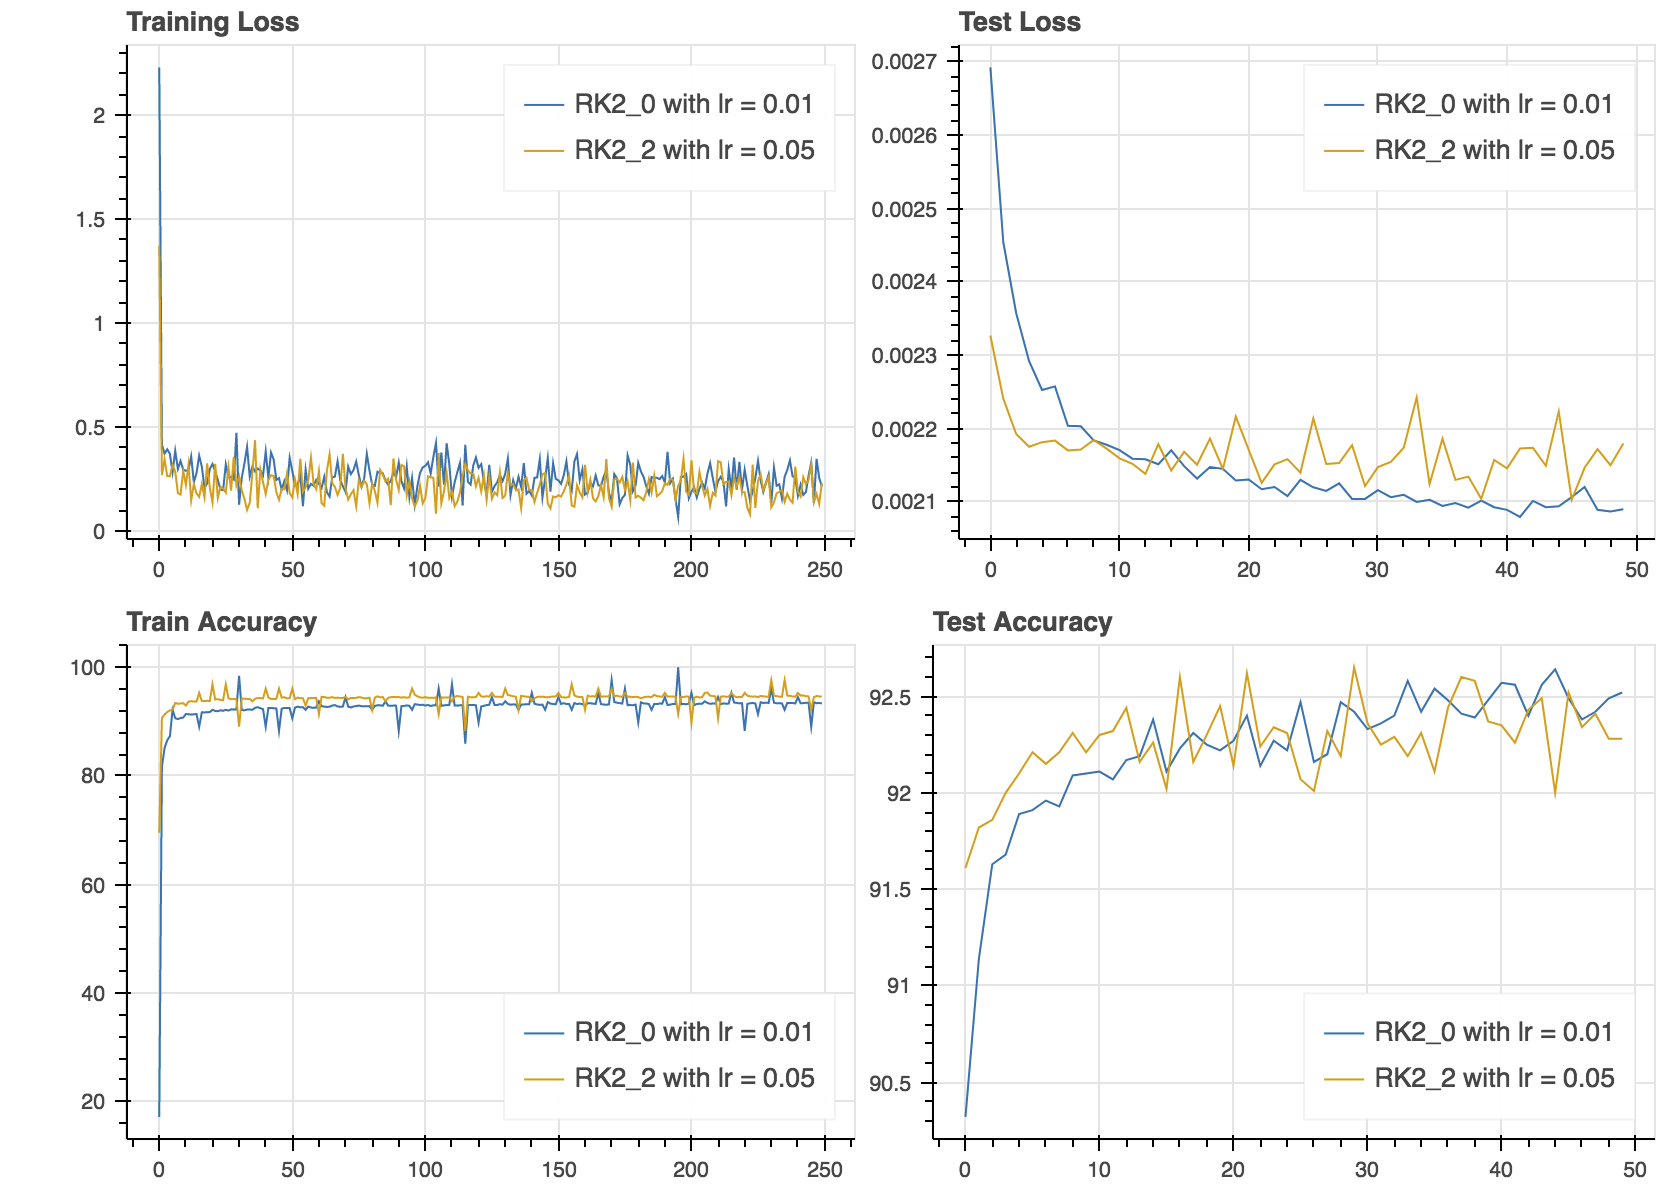
\includegraphics[scale=0.4]{lasso_4.png}
\\
Now, we show plots to compare our optimizer with simple
stochastic gradient descent and its variants.
\\
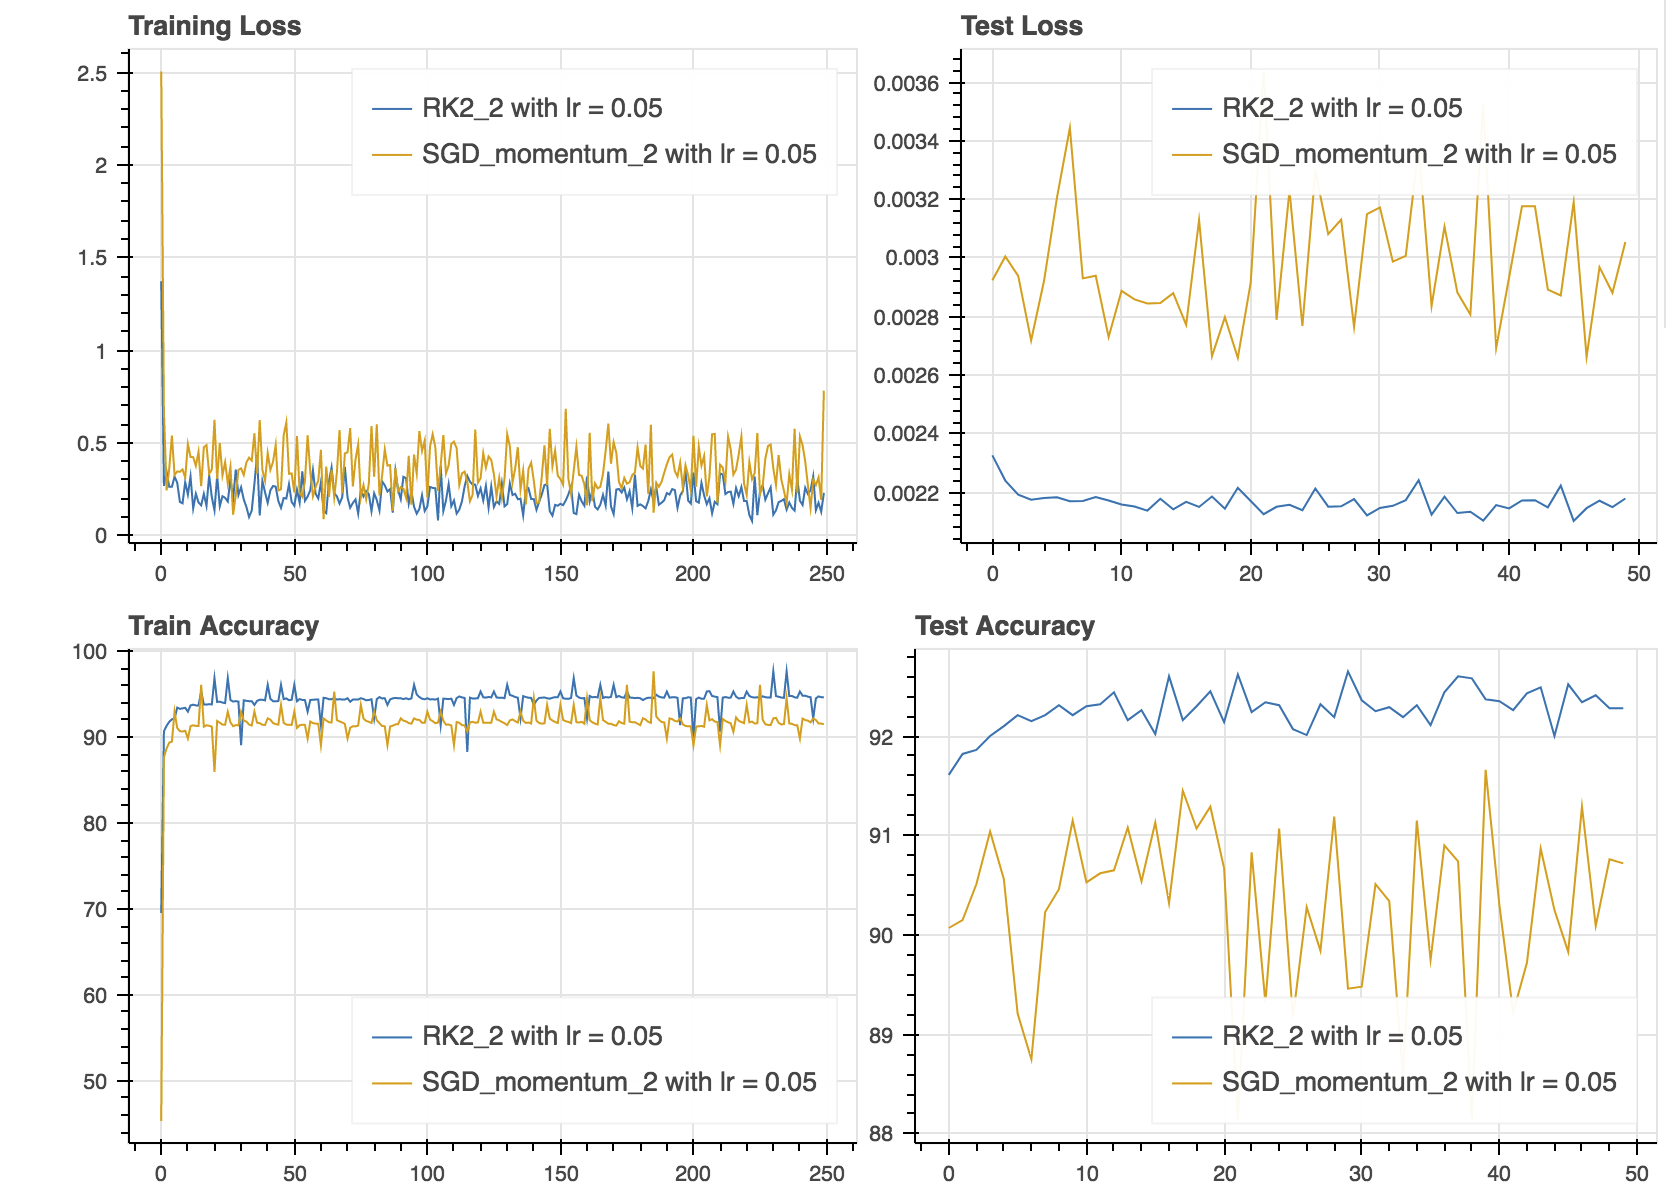
\includegraphics[scale=0.4]{lasso_3.png}
\\
Below we show plots to compare our optimizer with Accelerated
stochastic gradient descent.
% \\
% 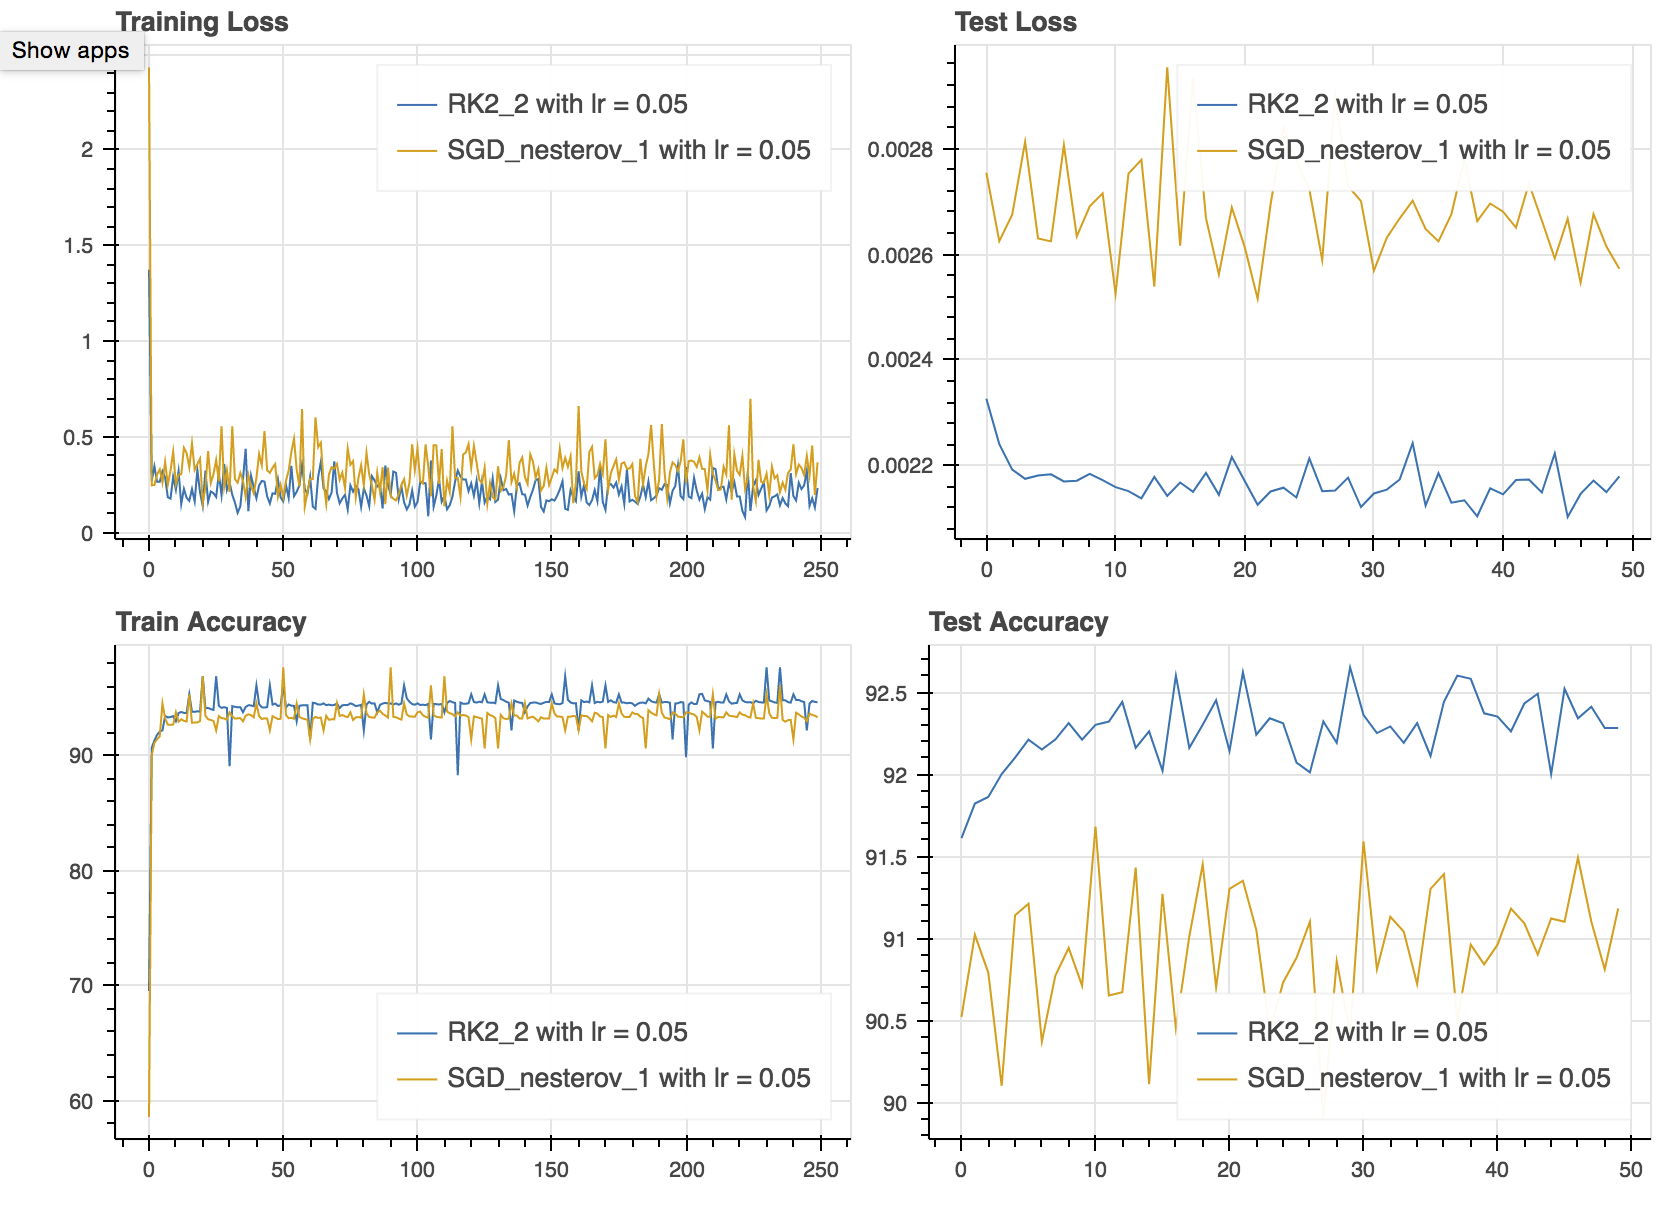
\includegraphics[scale=0.4]{lasso_2.png}
% \\
% Here we compare a 4th order optimizer based on Runge-Kutta
%Methods that we wrote with RK2 and SGD
\\
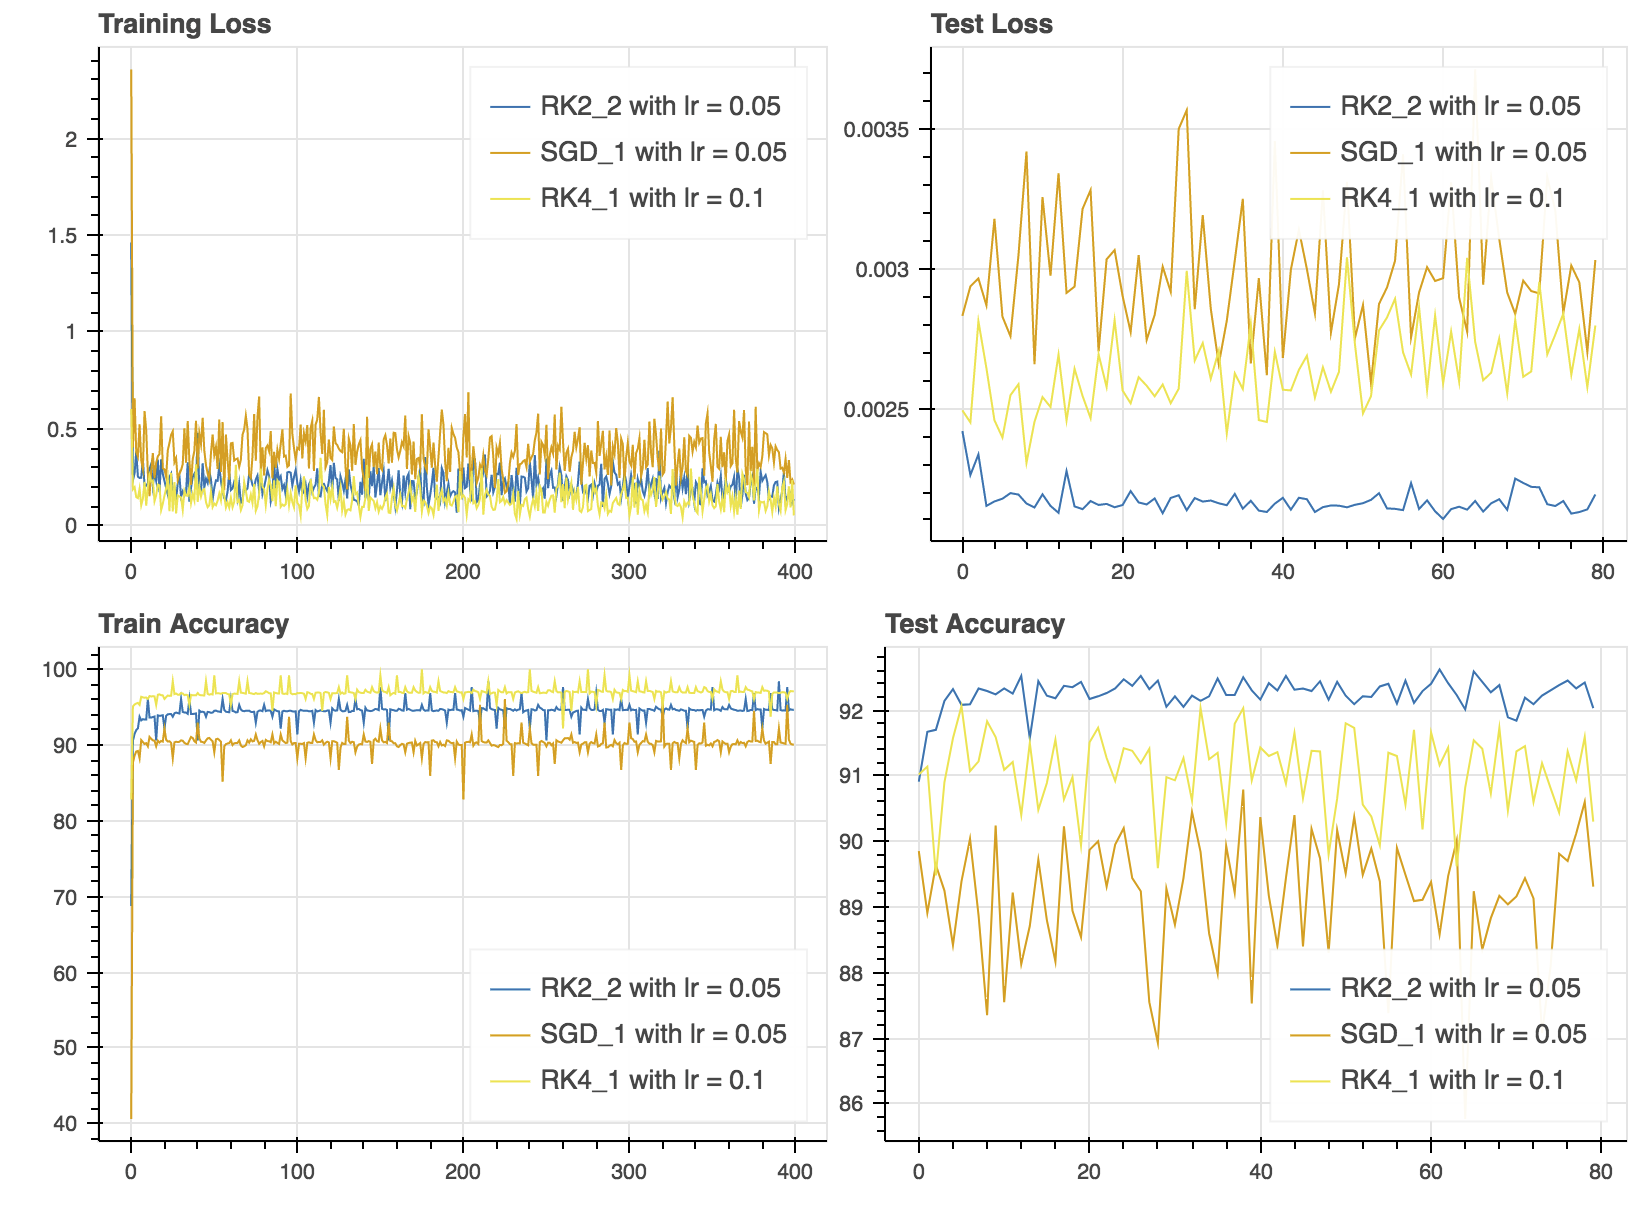
\includegraphics[scale=0.4]{lasso_1.png}
\\



\subsection{Deep Learning}

We experimented with the following setups
\begin{enumerate}
\item ResNet-18 on CIFAR-10 Dataset
\item ResNet-18 on Imagenet Dataset
\item WideResNet-16 on CIFAR-10
\item WideResNet-28 on CIFAR-10
\end{enumerate}

The table below shows that RK2 methods consistently achieve
the lowest training loss and highest training accuracy.
That is a constant feature we see across different models.
We make some observations in the next section
\begin{figure}[htb]
\centering
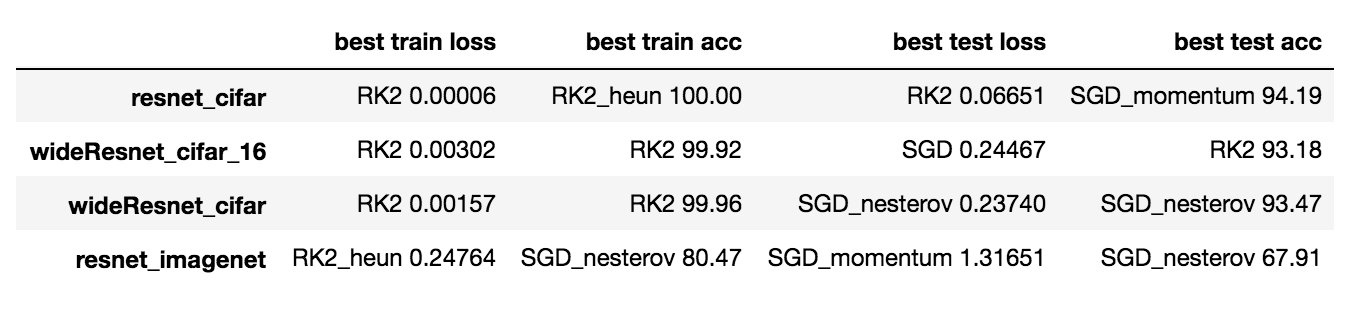
\includegraphics[scale=0.5]{non_param_test.png}
\caption{Overall Performance}
\label{fig:non_param_test}
\end{figure}


\subsection*{ResNet-18 on CIFAR-10}
Here we run the network with RK2 Ralston, RK2 Heun, SGD,
SGD with momentum and SGD with nesterov's momentum. We
ran the network with a wide variety of hyper-parameters
and here we saw that lower train loss translated to a
lower test loss.
\\
RK2 Ralston and RK2 Heun consistently achieve a lower
test loss than SGD and its variants. However, we notice
that the disparity between training and test loss for
RK2 is massive when compared to SGD.
% \begin{figure}[htb]
% 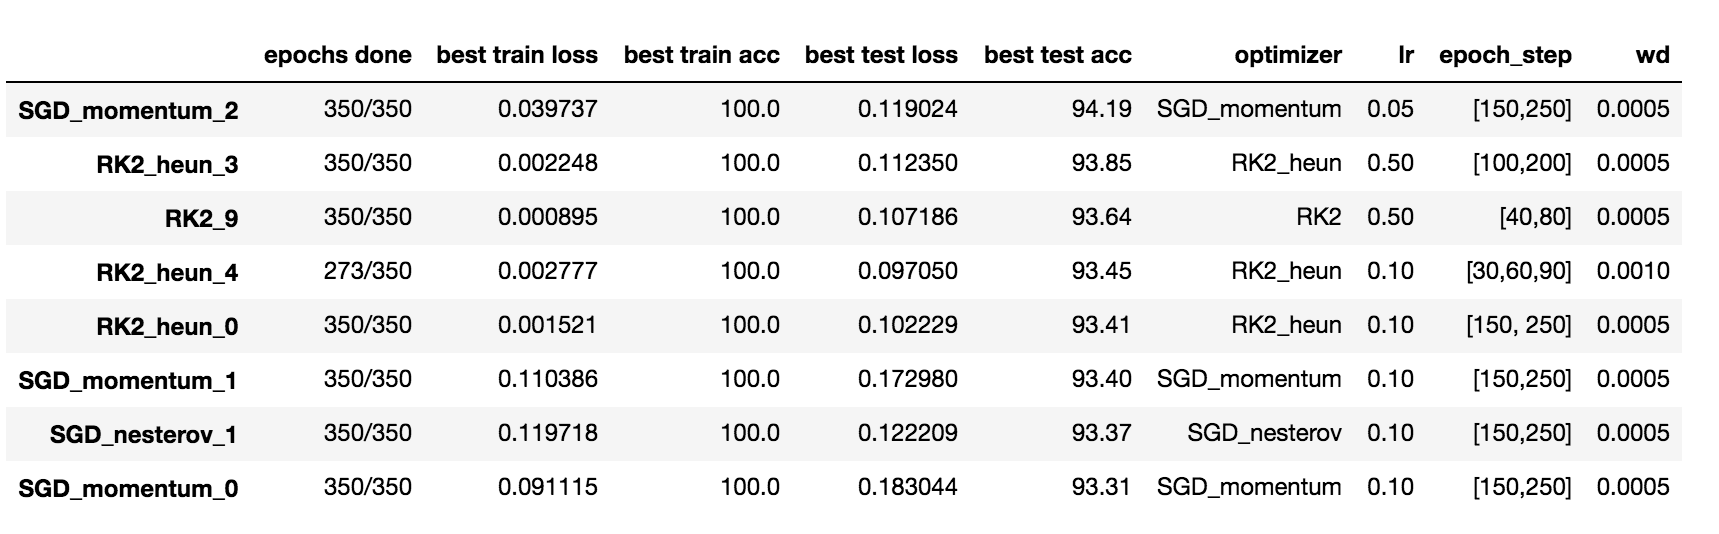
\includegraphics[scale=0.5]{cifar_resnet18_test_acc.png}
% \caption{CIFAR-10 Test Accuracy}
% \end{figure}

\begin{figure}[htb]
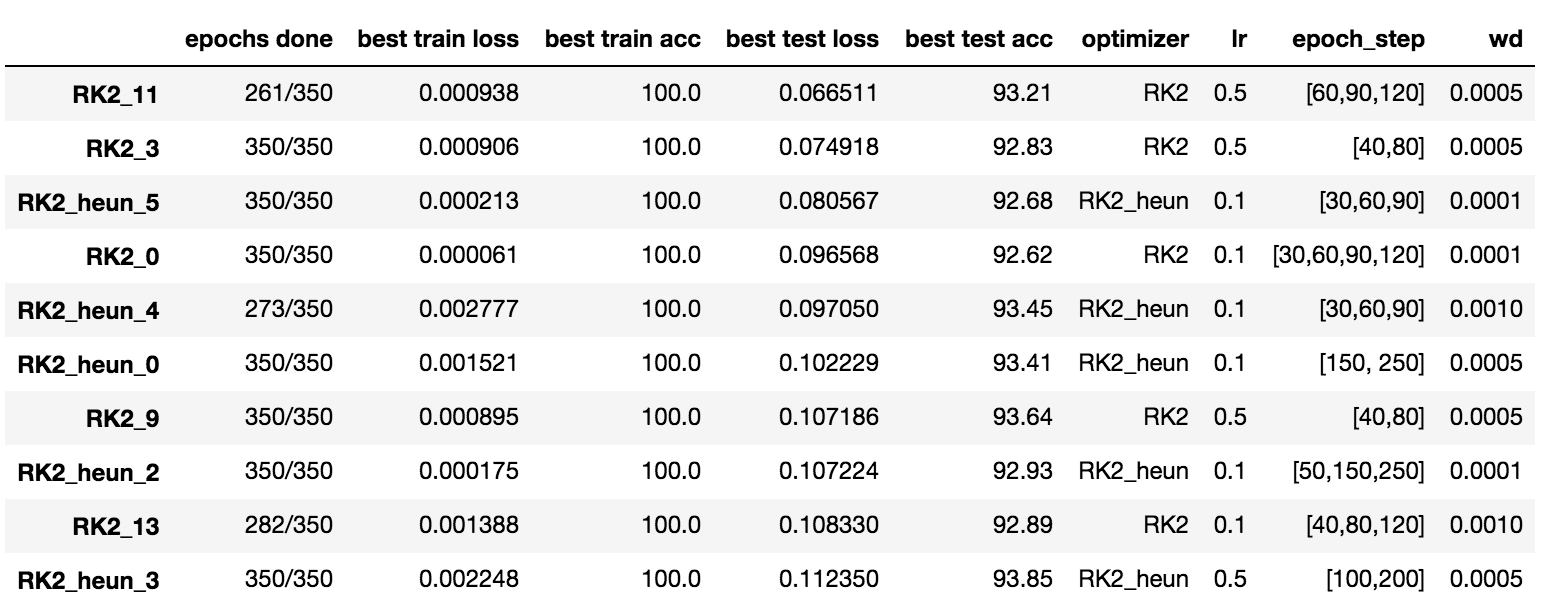
\includegraphics[scale=0.5]{cifar_resnet18_test_loss.png}
\caption{CIFAR-10 Test Loss}
\end{figure}


% \begin{figure}[htb]
% 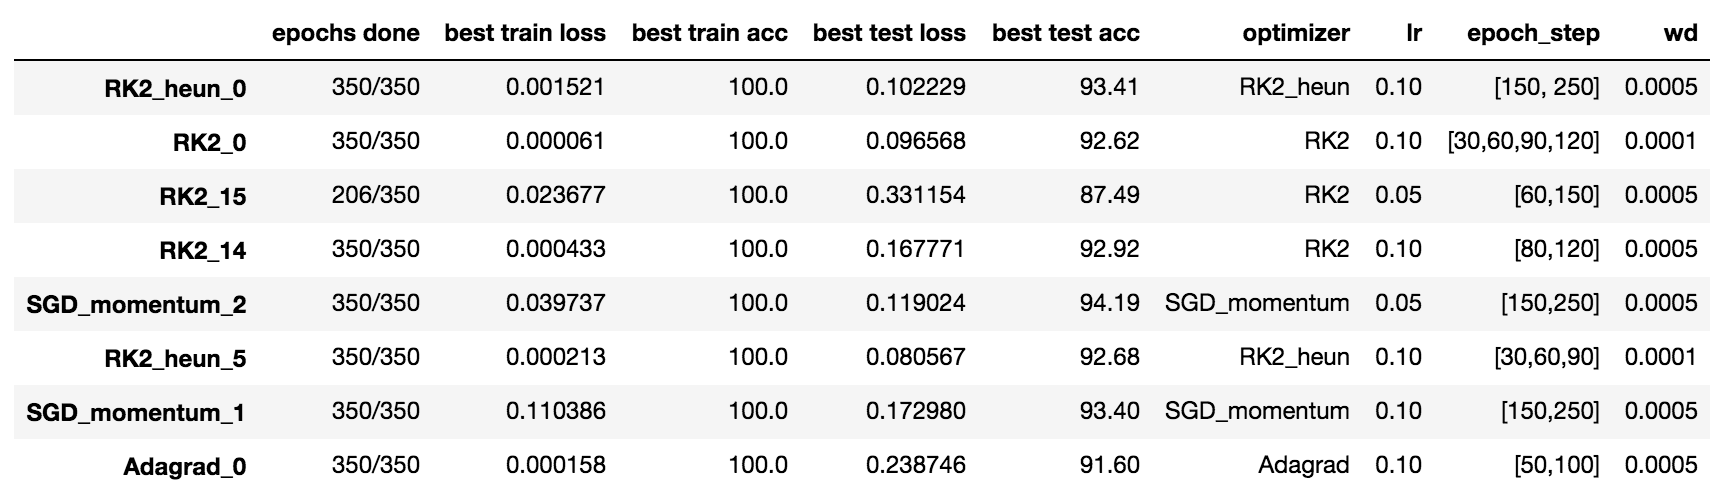
\includegraphics[scale=0.5]{cifar_resnet18_train_acc.png}
% \caption{CIFAR-10 Train Accuracy}
% \end{figure}

\begin{figure}[htb]
\begin{subfigure}{0.5\textwidth}
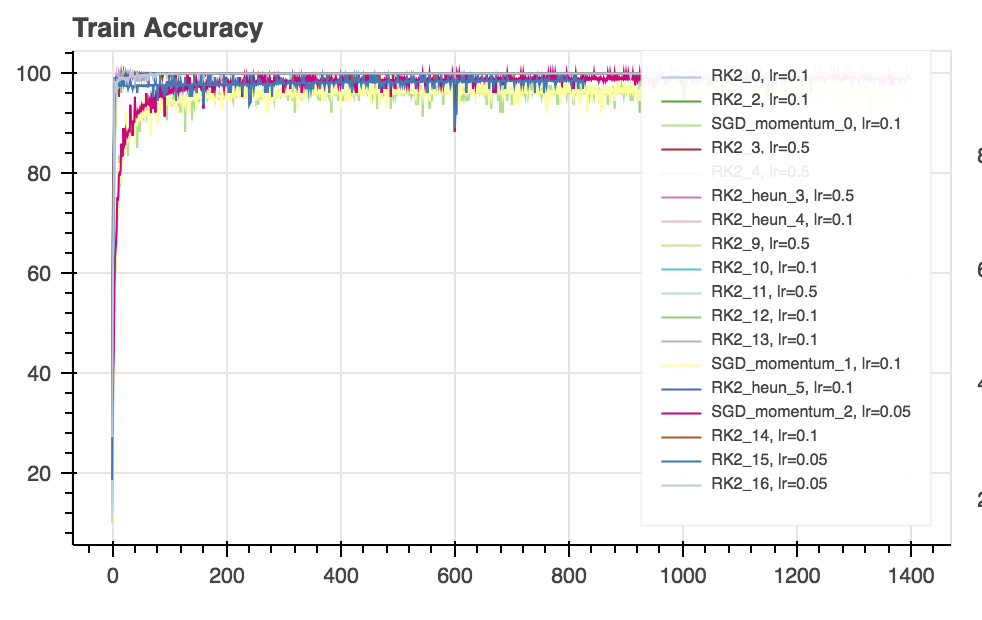
\includegraphics[scale=0.45]{plots/res_cifar.png}
\end{subfigure}
\begin{subfigure}{0.5\textwidth}
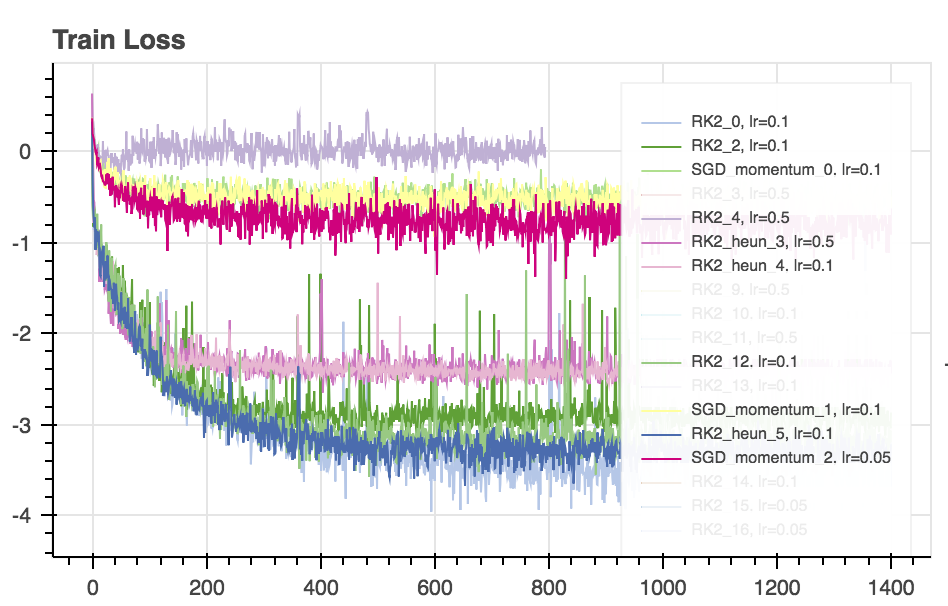
\includegraphics[scale=0.45]{plots/res_cifar_2.png}
\end{subfigure}
\begin{subfigure}{0.5\textwidth}
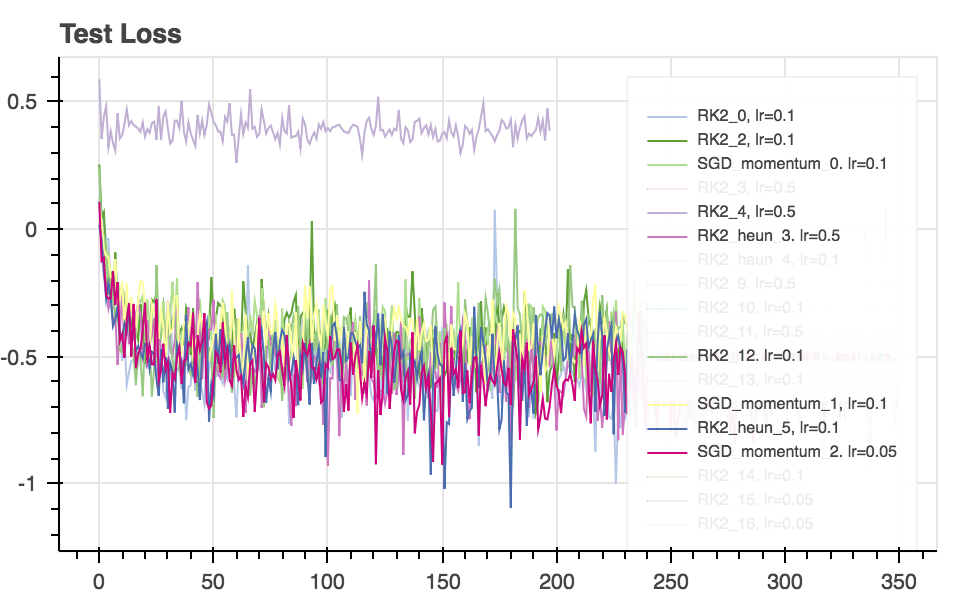
\includegraphics[scale=0.45]{plots/res_cifar_3.png}
\end{subfigure}
\begin{subfigure}{0.5\textwidth}
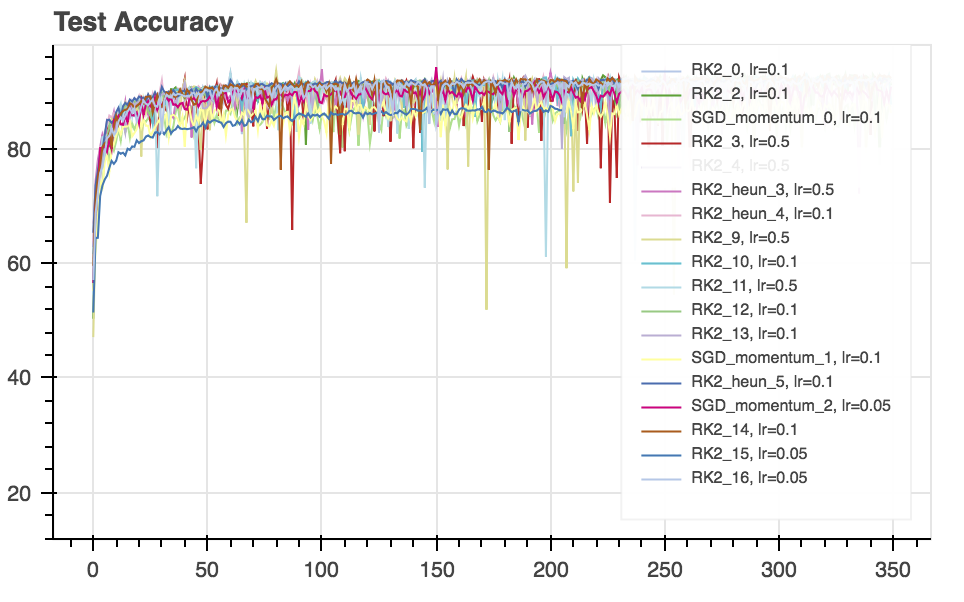
\includegraphics[scale=0.45]{plots/res_cifar_4.png}
\end{subfigure}

% 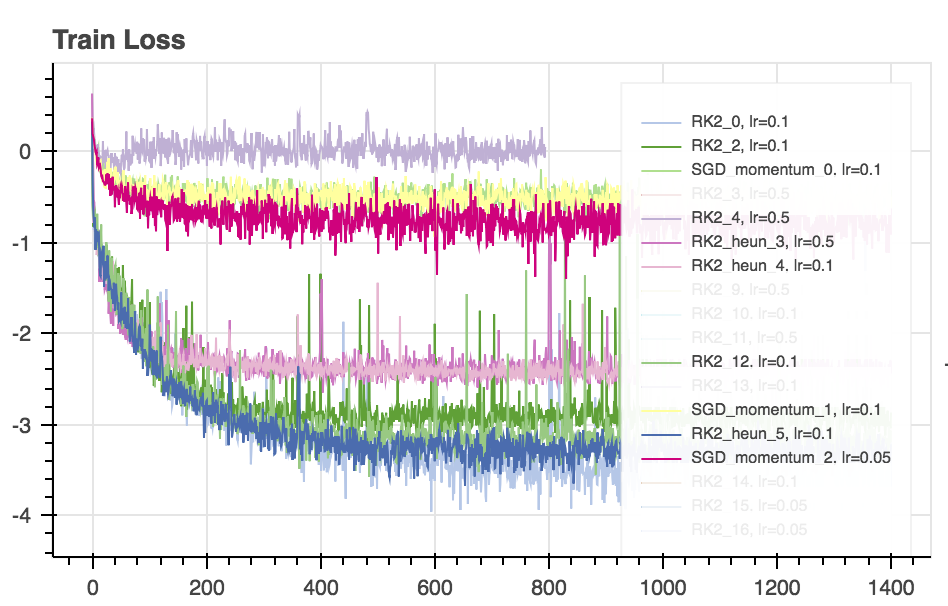
\includegraphics[scale=0.45]{plots/res_cifar_2.png}

% 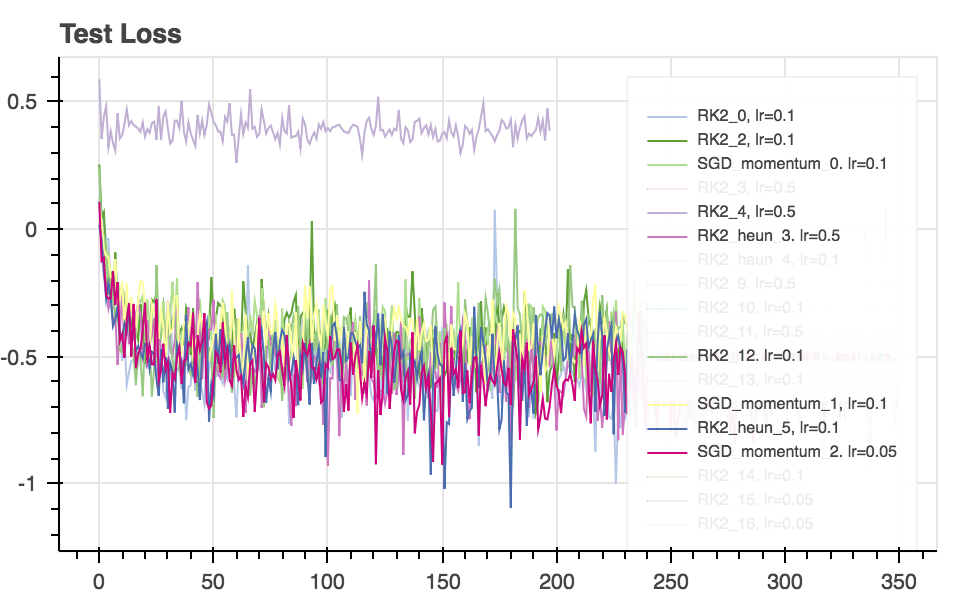
\includegraphics[scale=0.45]{plots/res_cifar_3.png}
% 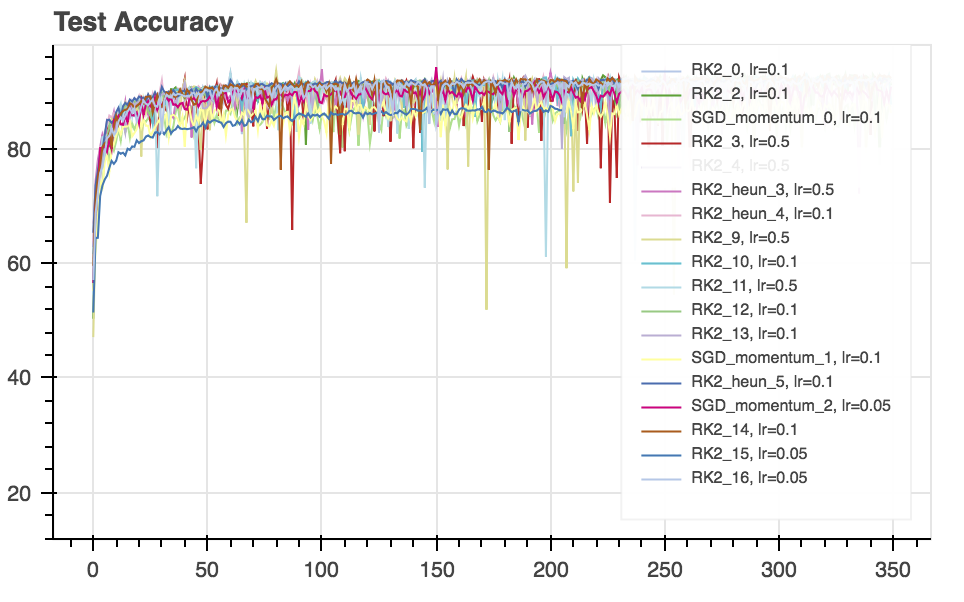
\includegraphics[scale=0.45]{plots/res_cifar_4.png}
\caption{Log-Loss Plot \& Accuracy : ResNet-18 on CIFAR-10}
\end{figure}




% \begin{figure}[htb]
% 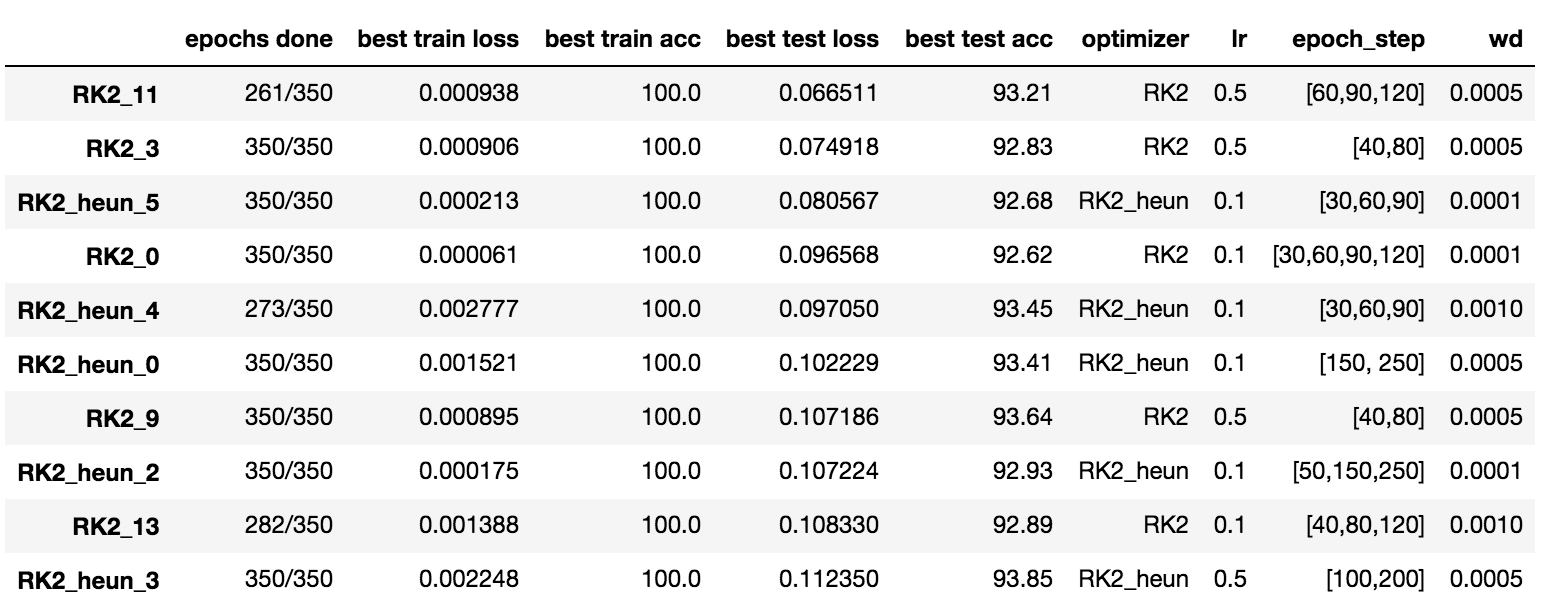
\includegraphics[scale=0.5]{cifar_resnet18_test_loss.png}
% \caption{CIFAR-10 Test Loss}
% \end{figure}

% \begin{figure}[htb]
% 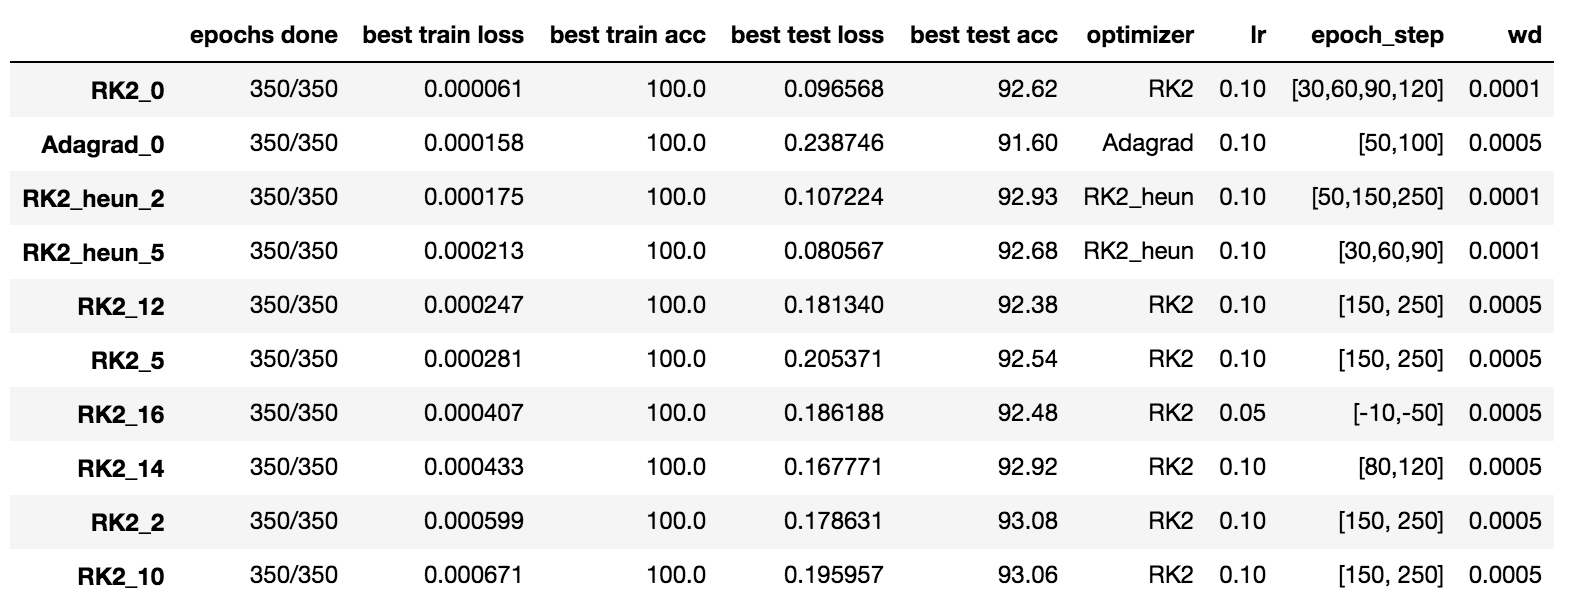
\includegraphics[scale=0.5]{cifar_resnet18_train_loss.png}
% \caption{CIFAR-10 Train loss}
% \end{figure}

\subsection*{ResNet-18 on Imagenet}
The results on ImageNet were also consistent with what
is seen across all models, RK2 consistently decay the
loss more than any other optimizer.
\\
\\
Here we experimented with a large number of Hyper-parameters
and another experiment we did here was to nor use batch
normalization. The exact effect of batch normalization on
optimization is not well known and we can see that its
presence can have a drastic effect on optimization.
\\
\\
Here we can see that with the same number of epochs, RK2
performs better but since it involves more computations,
if one looks at the wall-clock time SGD performs better
eventually.
% different experiments
\begin{figure}[htb]
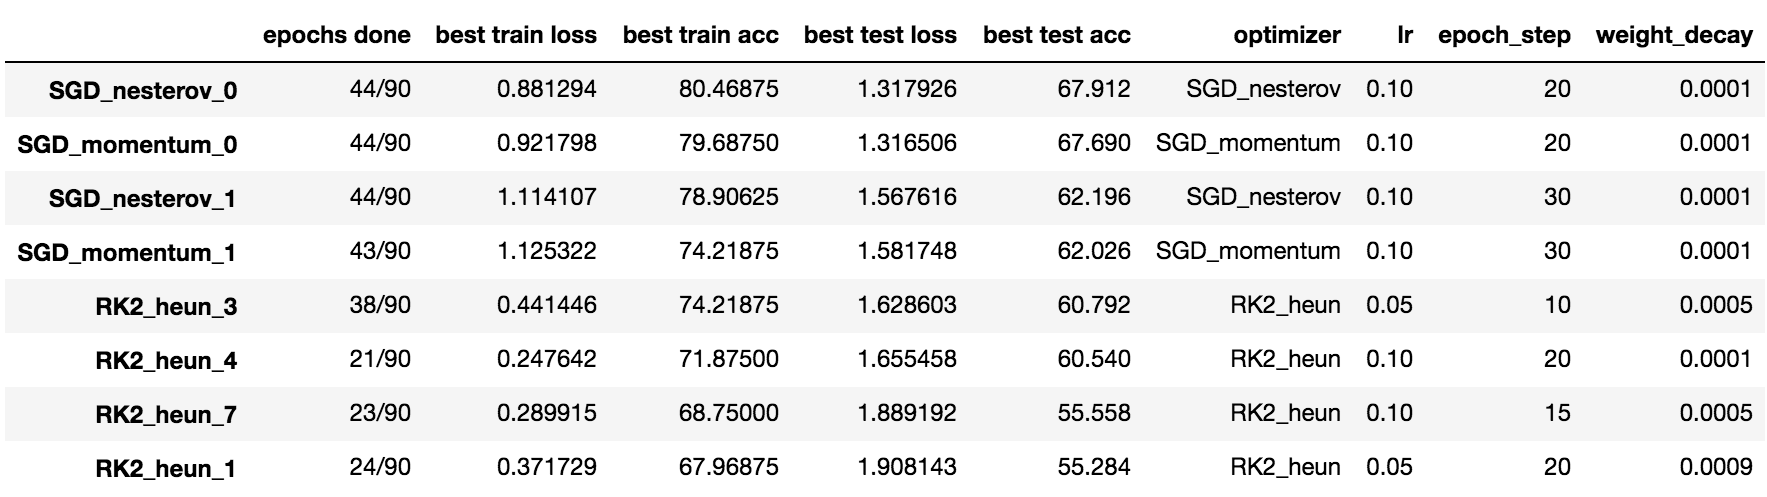
\includegraphics[scale=0.5]{imagenet_resnet18_test_acc.png}
\caption{Imagenet Test Accuracy}
\end{figure}

\begin{figure}[htb]
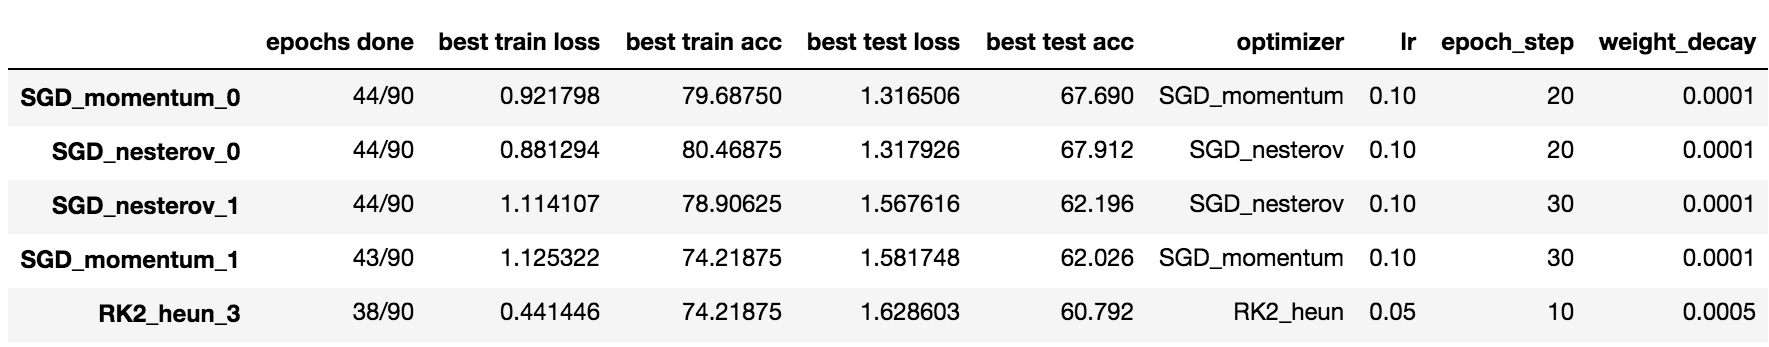
\includegraphics[scale=0.5]{imagenet_resnet18_test_loss.png}
\caption{Imagenet Test Loss}
\end{figure}

\begin{figure}[htb]
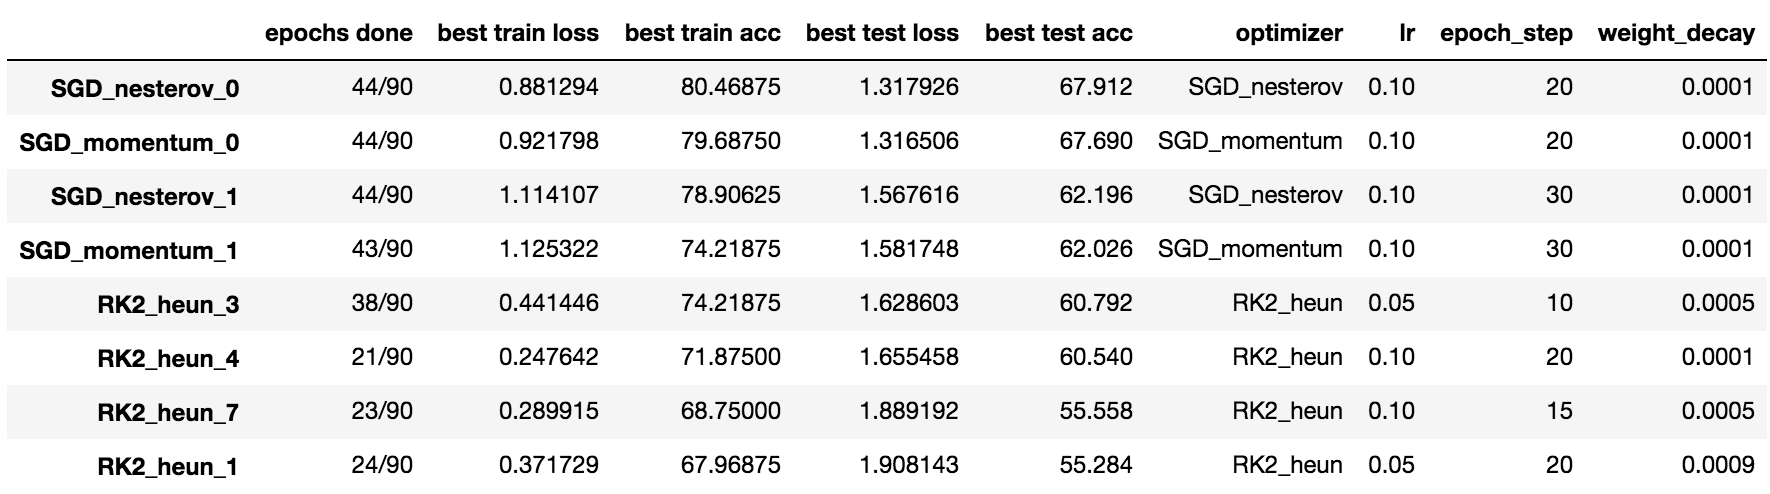
\includegraphics[scale=0.5]{imagenet_resnet18_train_acc.png}
\caption{Imagenet Train Accuracy}
\end{figure}

\begin{figure}[htb]
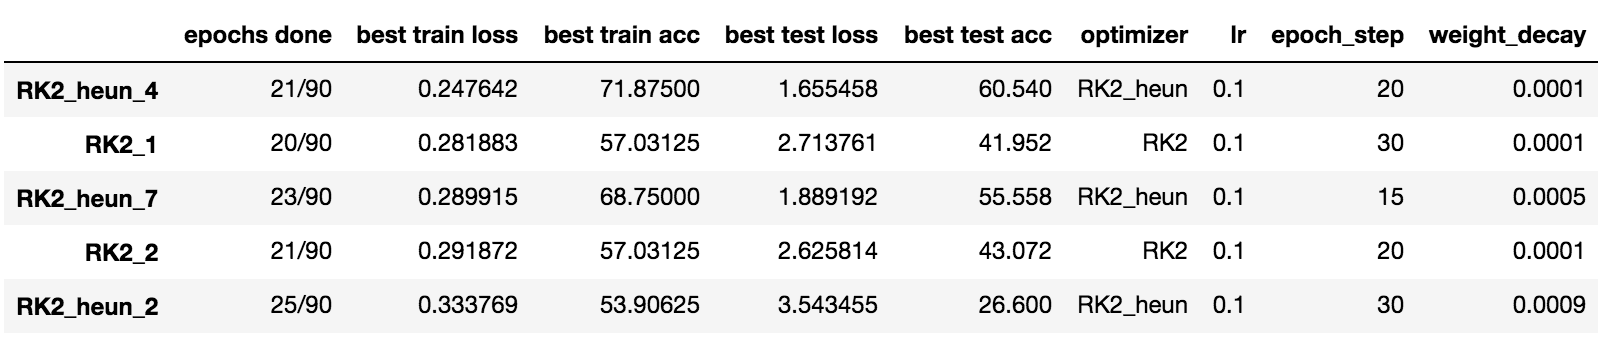
\includegraphics[scale=0.5]{imagenet_resnet18_train_loss.png}
\caption{Imagenet Test Loss}
\end{figure}

\begin{figure}[htb]
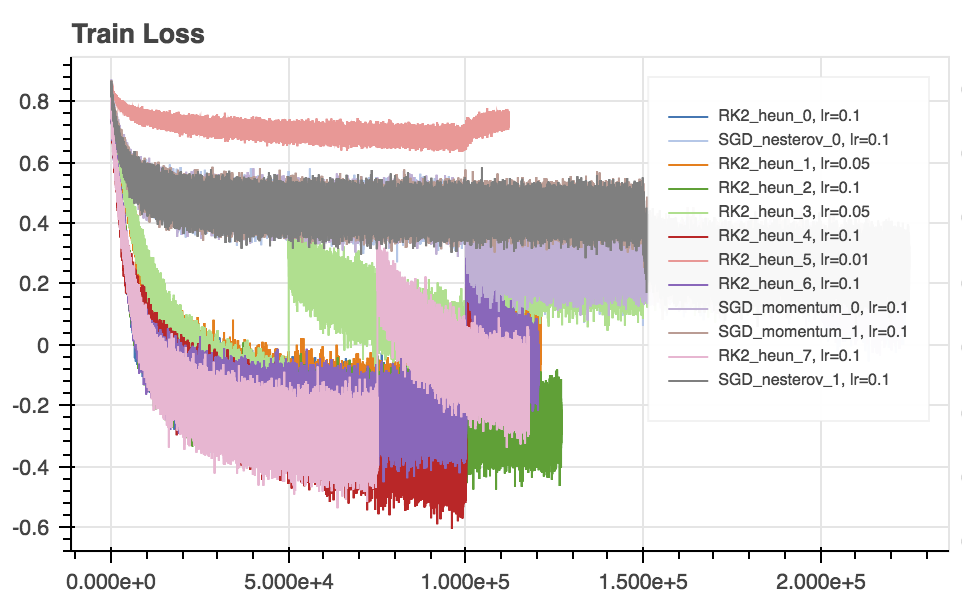
\includegraphics[scale=0.5]{plots/imagenet.png}
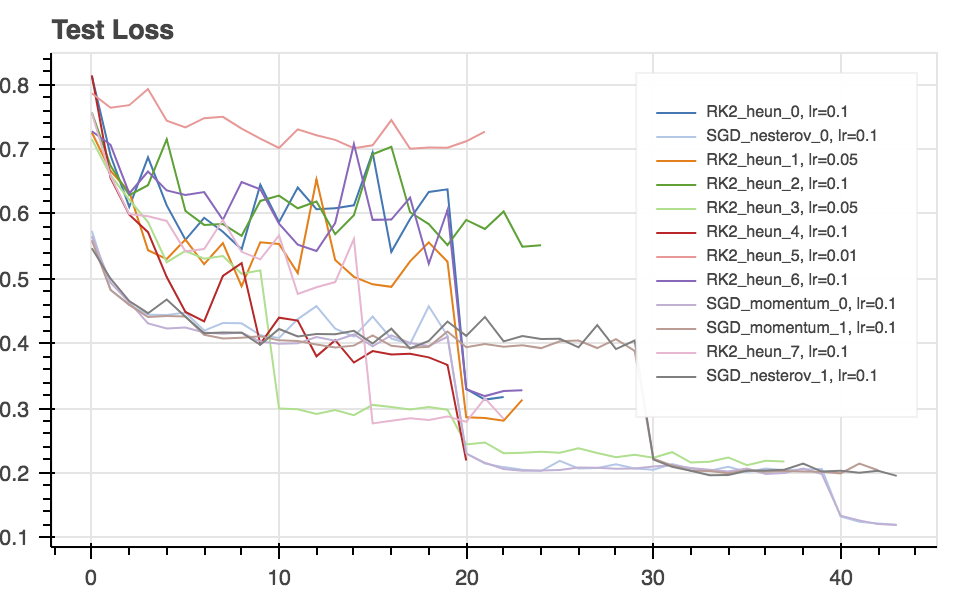
\includegraphics[scale=0.5]{plots/imagenet_1.png}
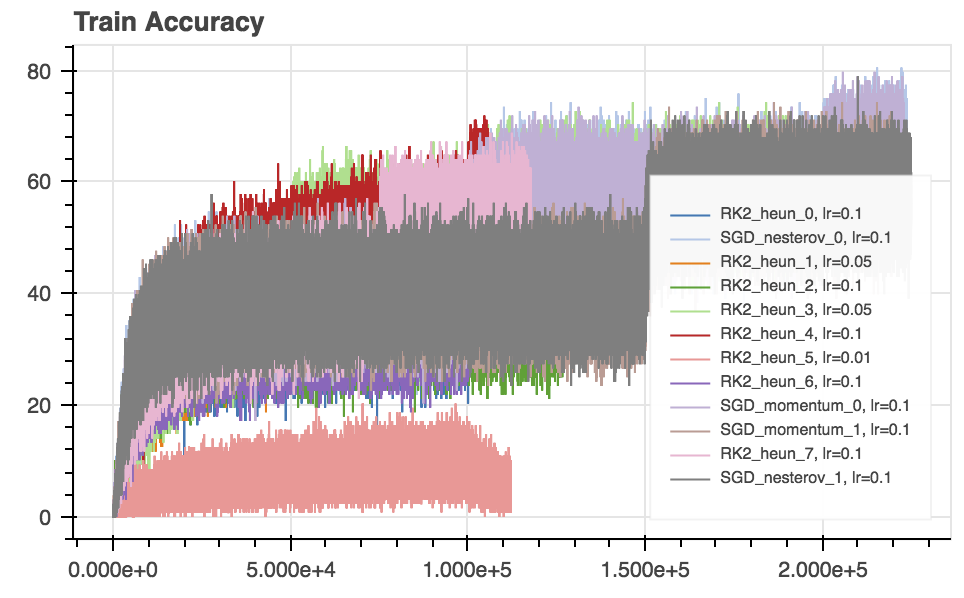
\includegraphics[scale=0.5]{plots/imagenet_2.png}
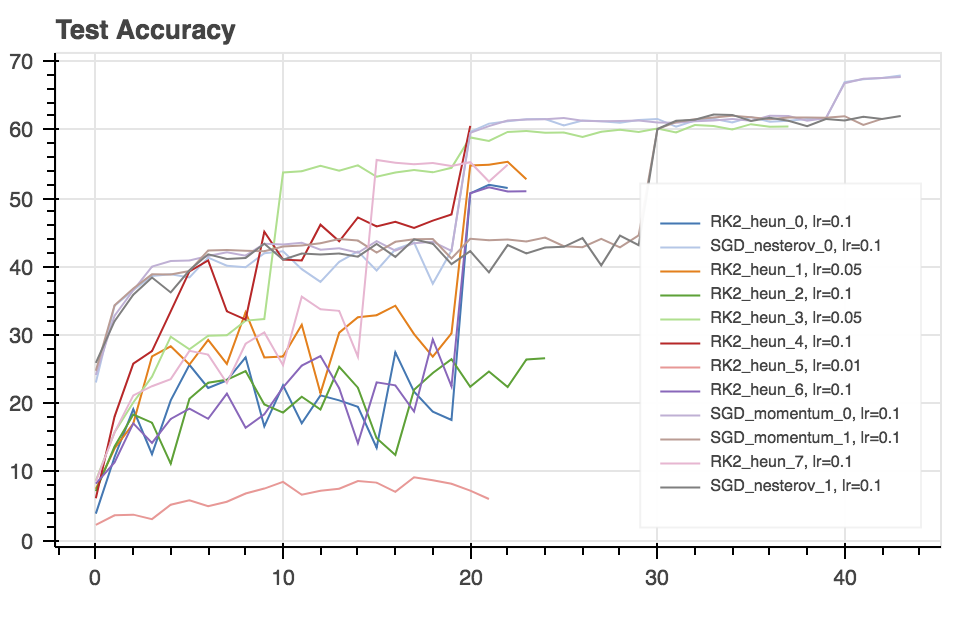
\includegraphics[scale=0.5]{plots/imagenet_3.png}


\caption{Log-Loss Plot \& Accuracy : ResNet-18 on ImageNet}
\end{figure}



% \subsection*{WideResNet-16 on CIFAR-10}

\begin{figure}[htb]
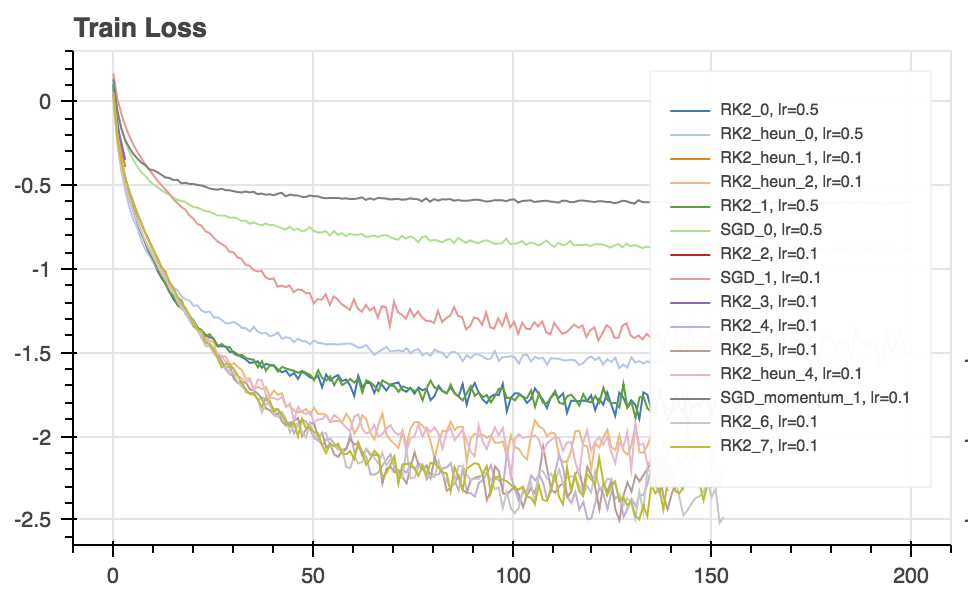
\includegraphics[scale=0.5]{plots/wide_resnet16.png}
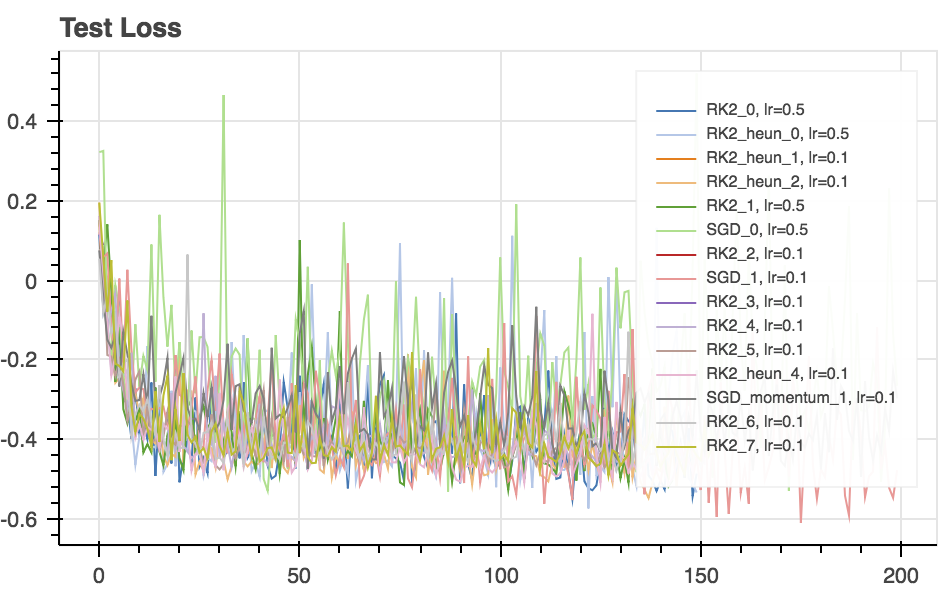
\includegraphics[scale=0.5]{plots/wide_resnet16_1.png}
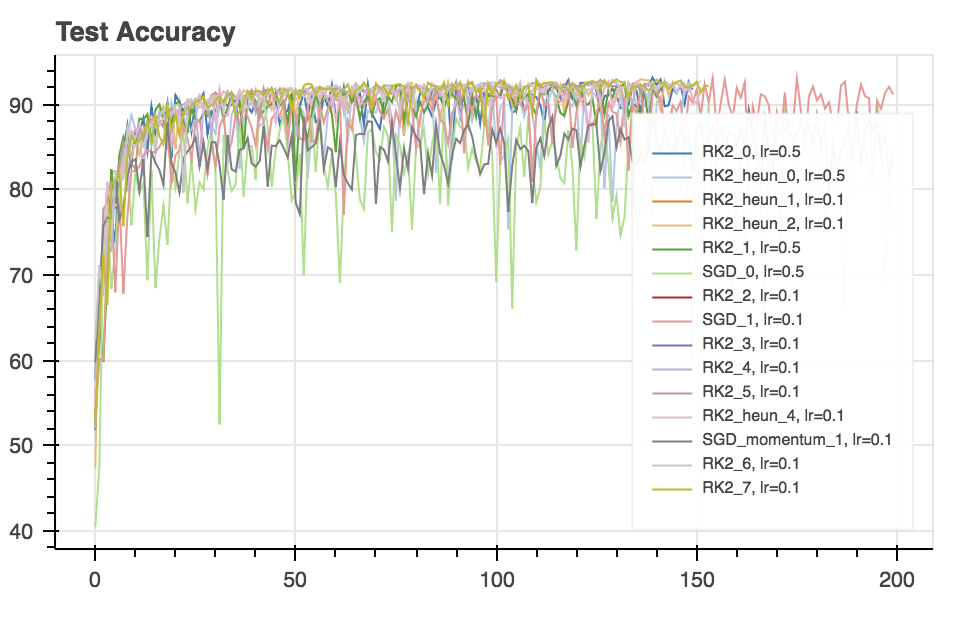
\includegraphics[scale=0.5]{plots/wide_resnet16_2.png}
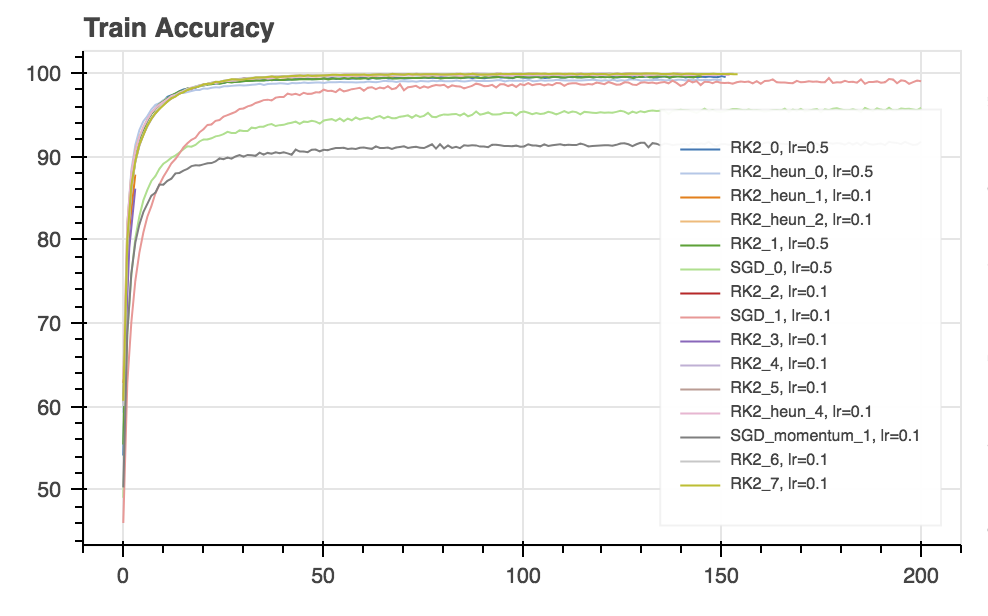
\includegraphics[scale=0.5]{plots/wide_resnet16_3.png}


\caption{Log-Loss Plot \& Accuracy : WideResNet-16 on CIFAR-10}
\end{figure}

\section{Conclusion}
We notice that Runge-Kutta methods when used as optimizers
perform significantly better thqn Stochqstic Gradient
Descent, however we do not see this perforance directly
translated in the peroformance. This however is an open
area of research, understanding generalization ability
of neural networks.

% \begin{figure}[htb]
% 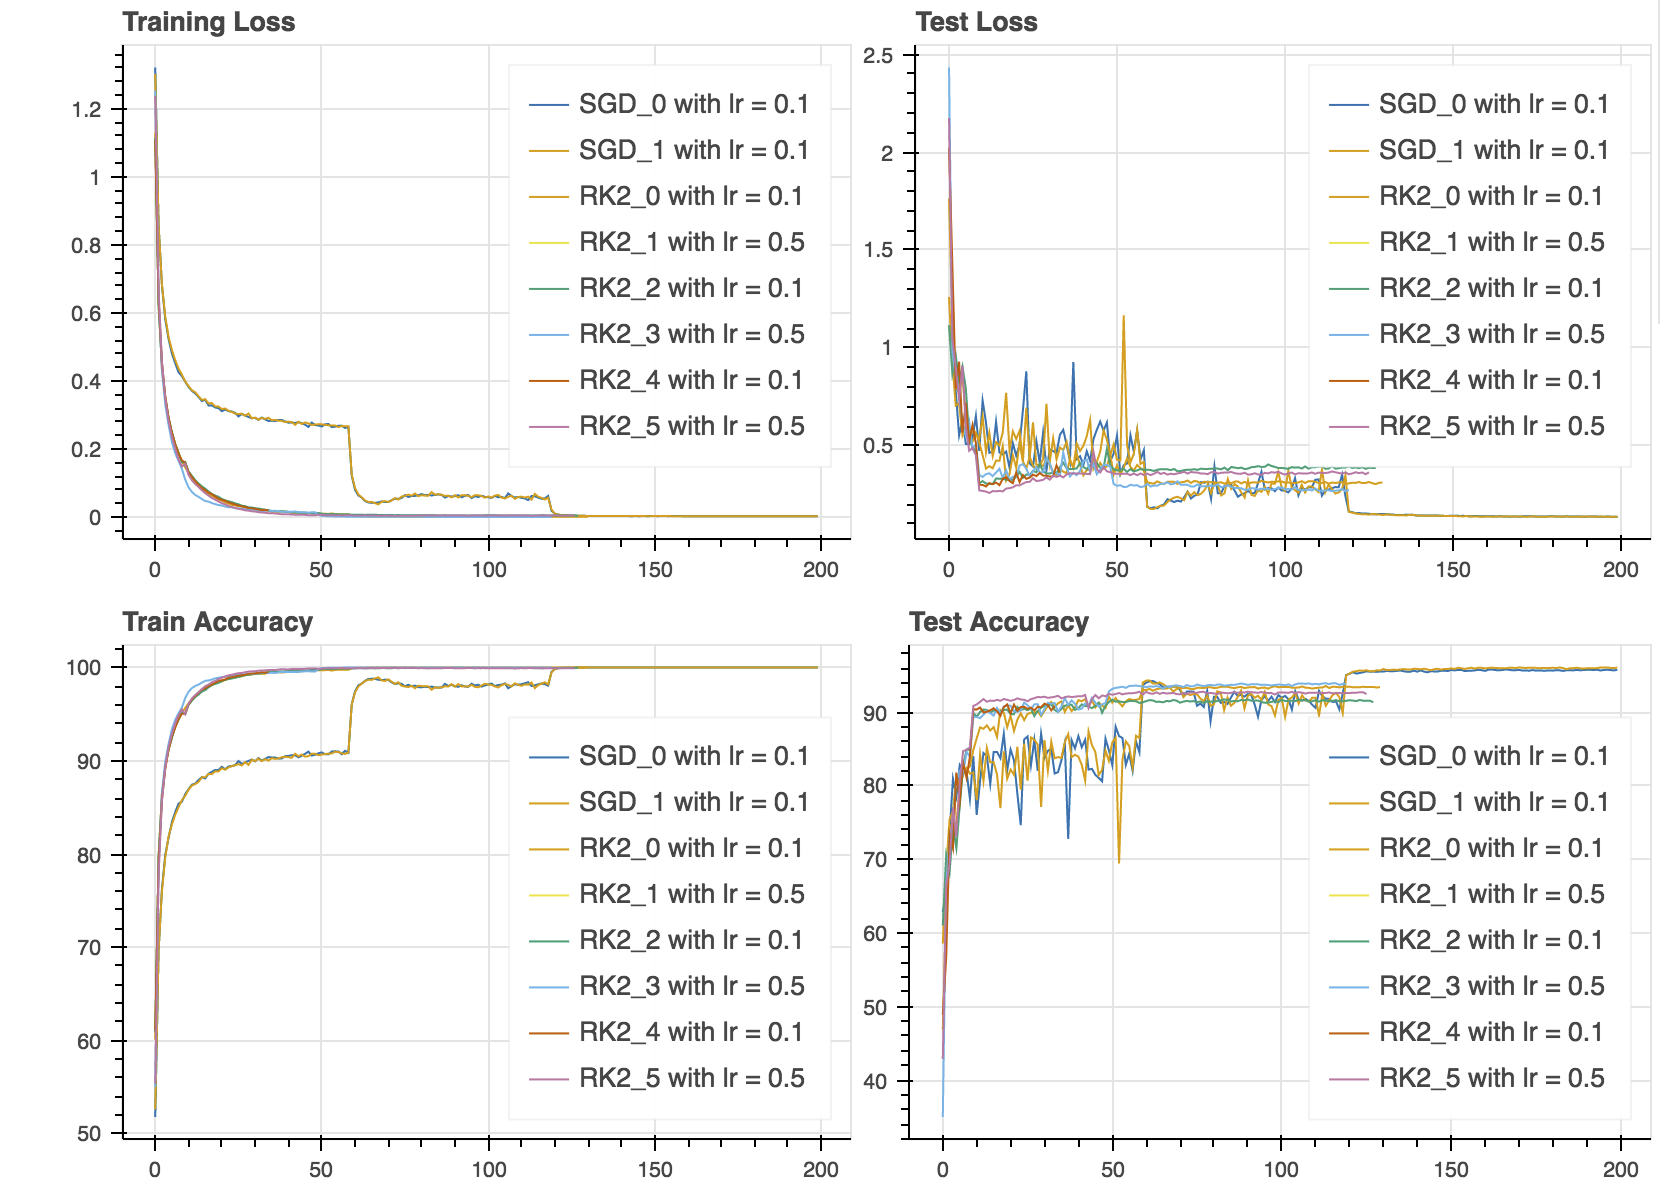
\includegraphics[scale=0.5]{wideresnet.png}
% \caption{WideResNet-16 on CIFAR-10}
% \end{figure}


% \begin{figure}[htb]
% 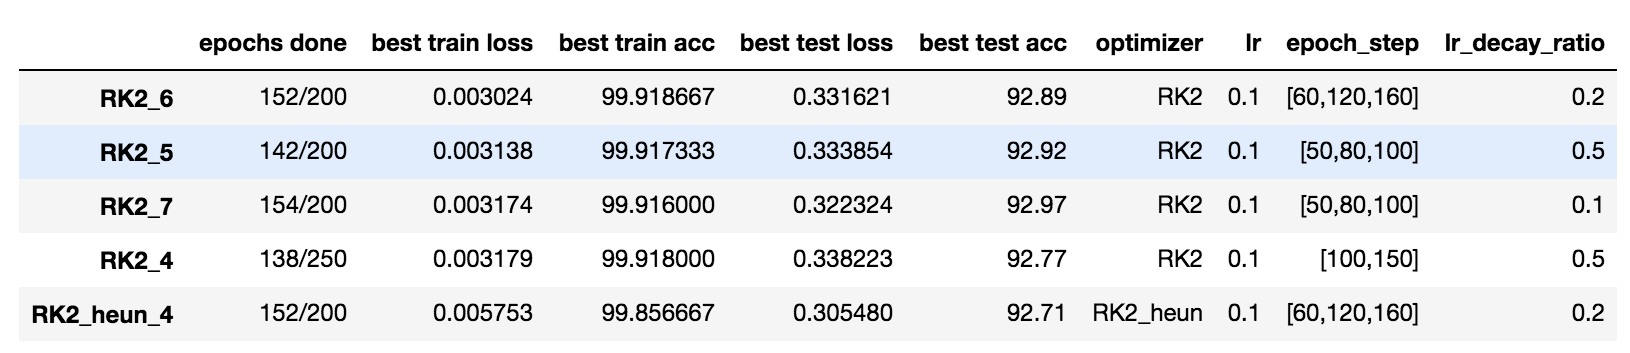
\includegraphics[scale=0.5]{wideresnet16_train_loss.png}
% \caption{WideResNet-16 CIFAR-10 Train loss}
% \end{figure}

% \begin{figure}[htb]
% 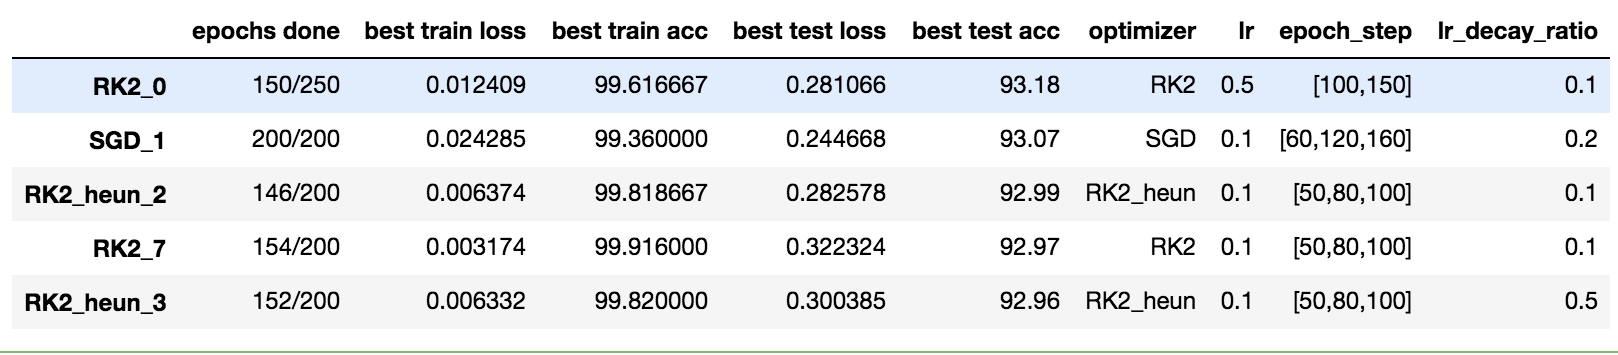
\includegraphics[scale=0.5]{wideresnet16_test_acc.png}
% \caption{WideResNet-16 CIFAR-10 Test Accuracy}
% \end{figure}


% \begin{figure}[htb]
% 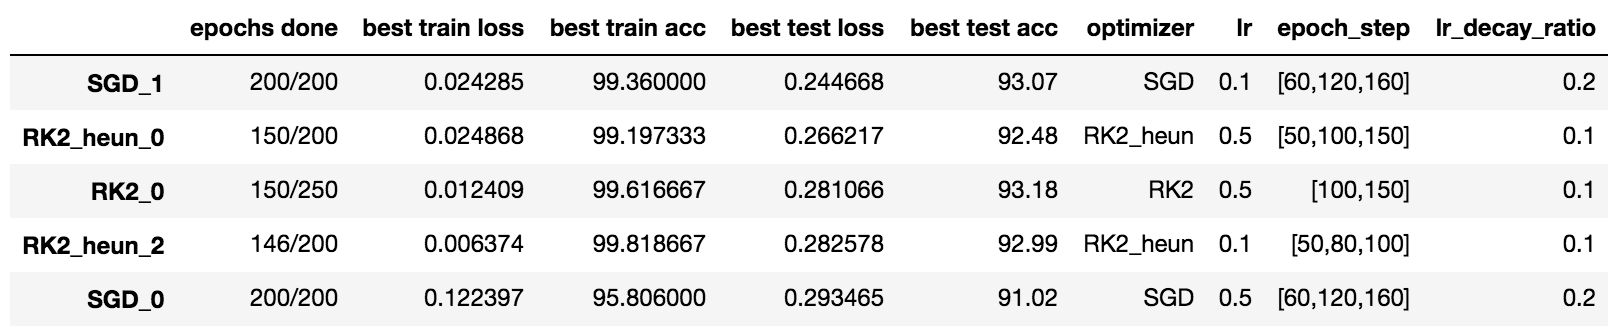
\includegraphics[scale=0.5]{wideresnet16_test_loss.png}
% \caption{WideResNet-16 CIFAR-10 Test loss}
% \end{figure}

% \begin{figure}[htb]
% 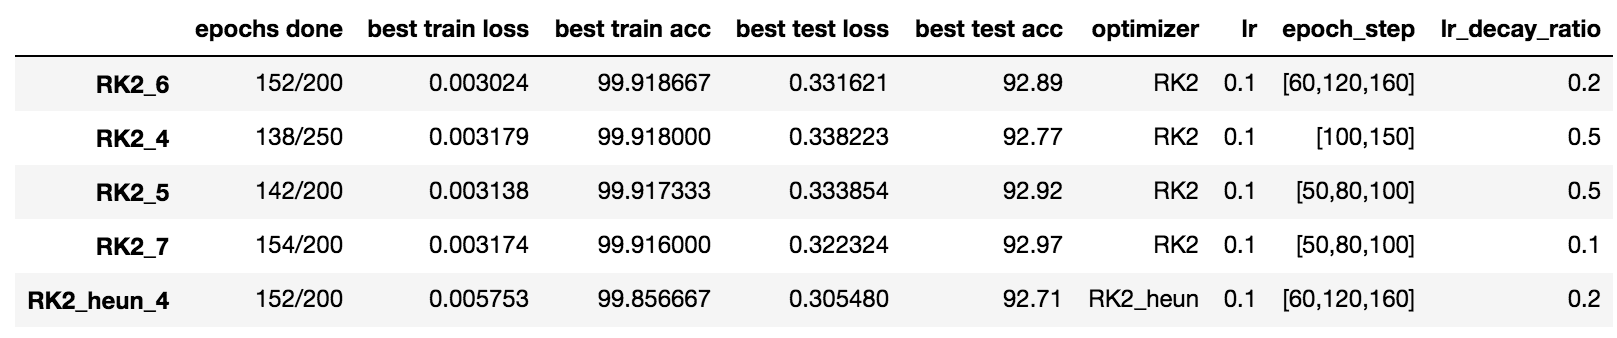
\includegraphics[scale=0.5]{wideresnet16_train_acc.png}
% \caption{WideResNet-16 CIFAR-10 Train Accuracy}
% \end{figure}

% \subsection*{WideResNet-28 on CIFAR-10}

\begin{figure}[htb]
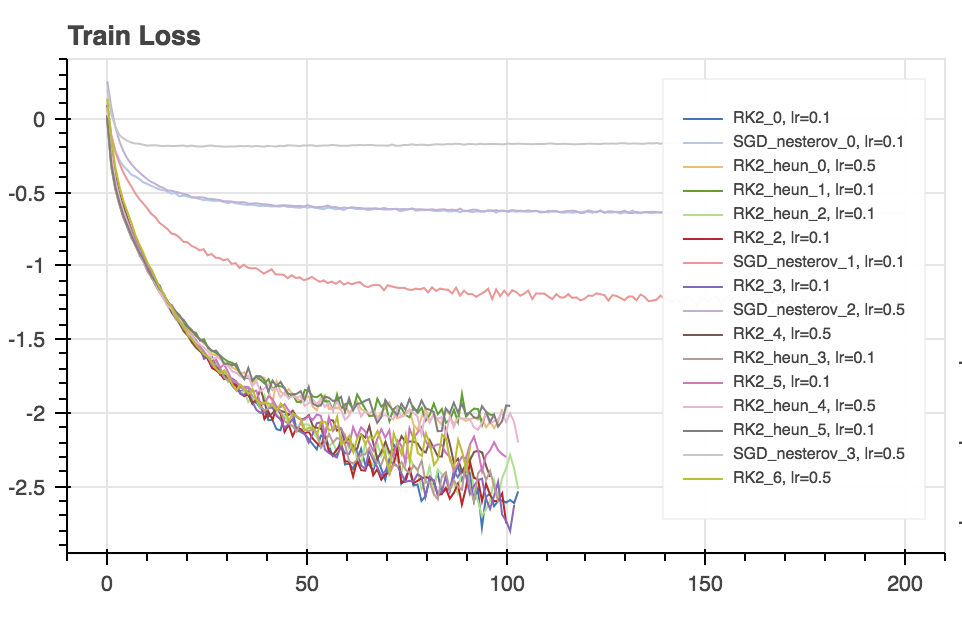
\includegraphics[scale=0.5]{plots/wide_resnet28.png}
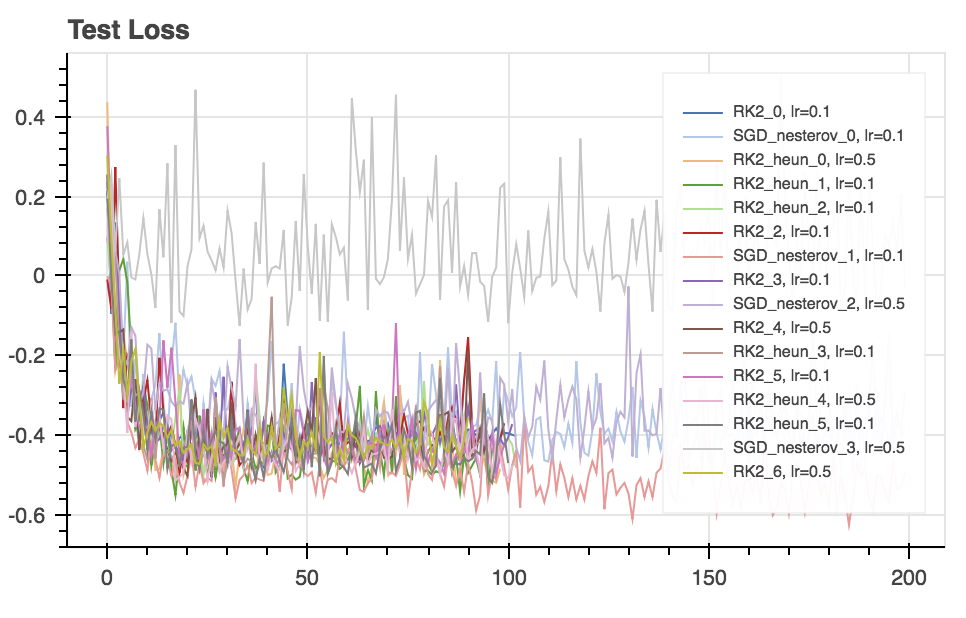
\includegraphics[scale=0.5]{plots/wide_resnet28_1.png}
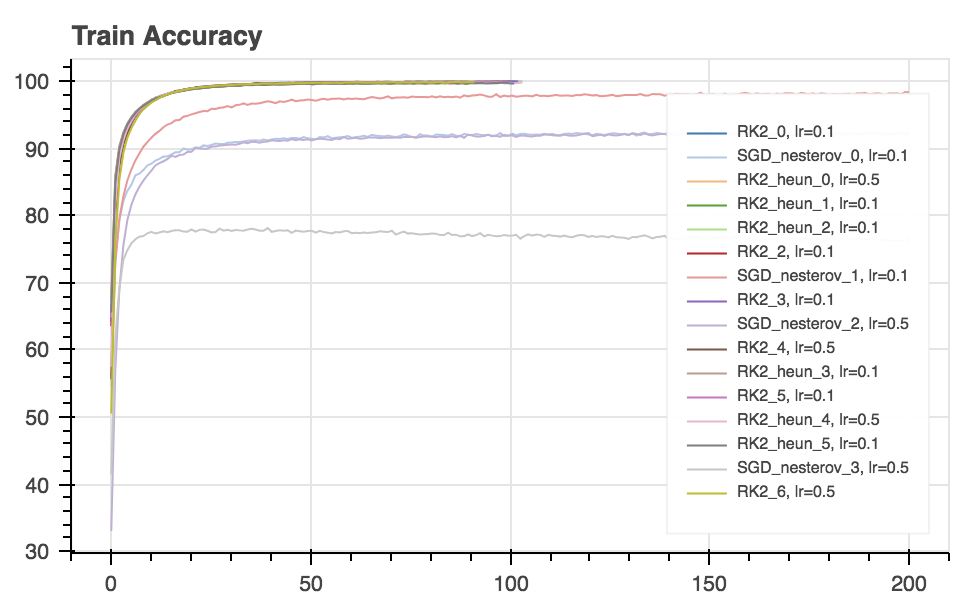
\includegraphics[scale=0.5]{plots/wide_resnet28_2.png}
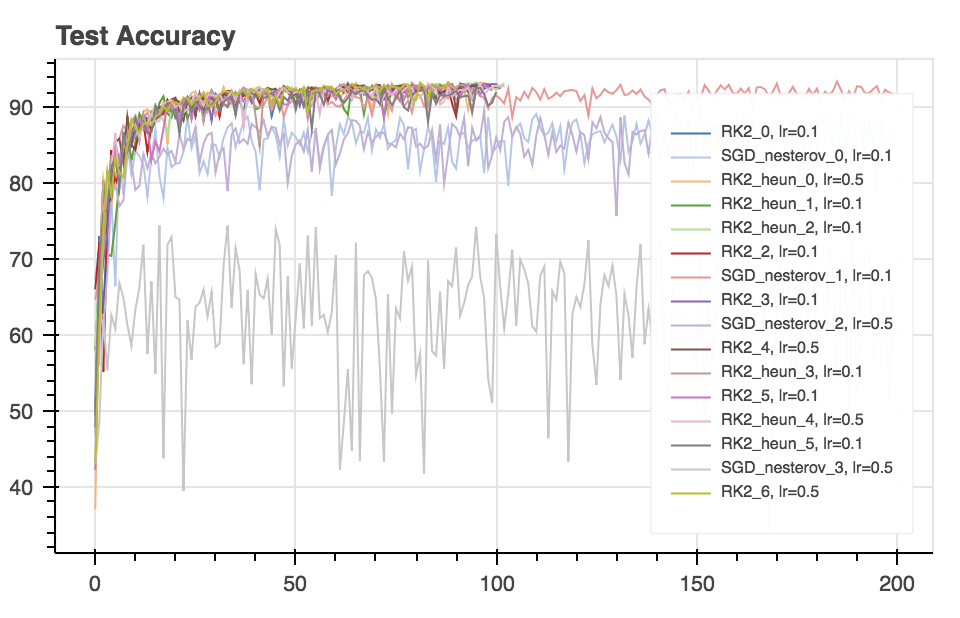
\includegraphics[scale=0.5]{plots/wide_resnet28_3.png}
\caption{Log-Loss Plot \& Accuracy : WideResNet-28 on CIFAR-10}
\end{figure}

% \begin{figure}[htb]
% 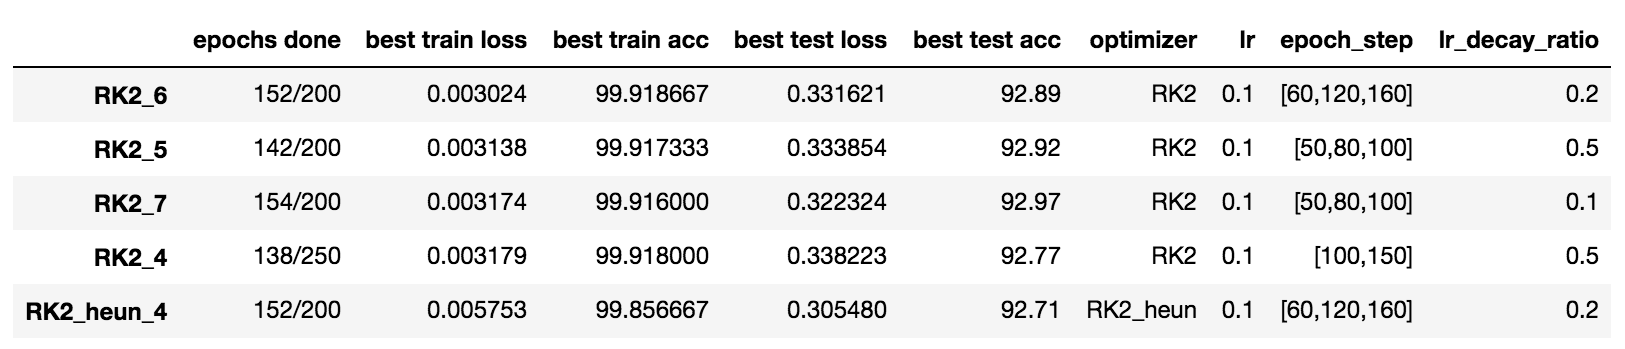
\includegraphics[scale=0.5]{wideresnet28_train_loss.png}
% \caption{WideResNet-28 CIFAR-10 Train loss}
% \end{figure}

% \begin{figure}[htb]
% 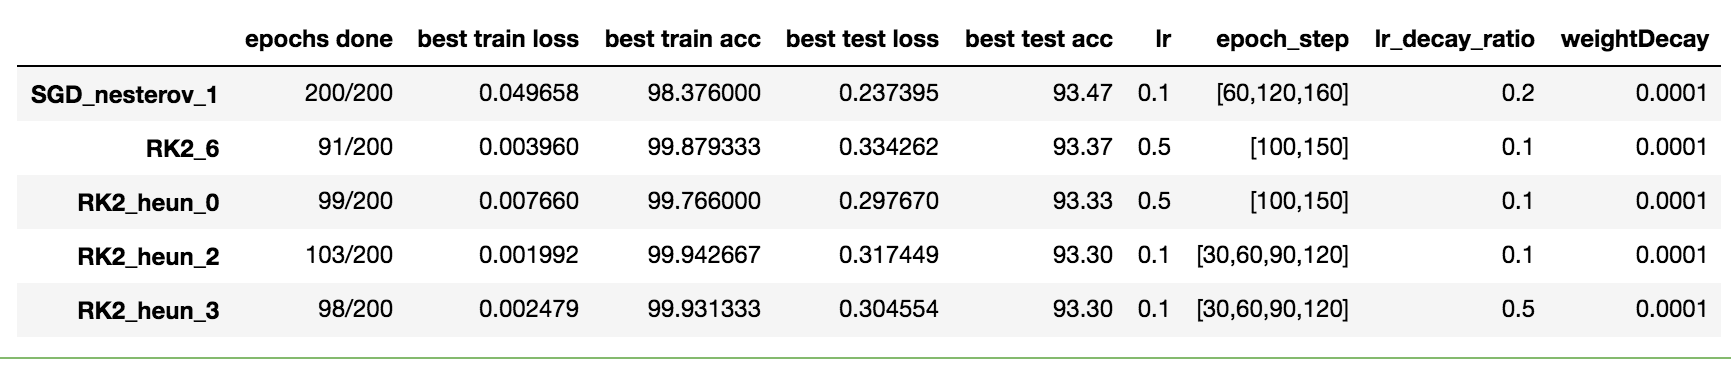
\includegraphics[scale=0.5]{wideresnet28_test_acc.png}
% \caption{WideResNet-28 CIFAR-10 Test Accuracy}
% \end{figure}


% \begin{figure}[htb]
% 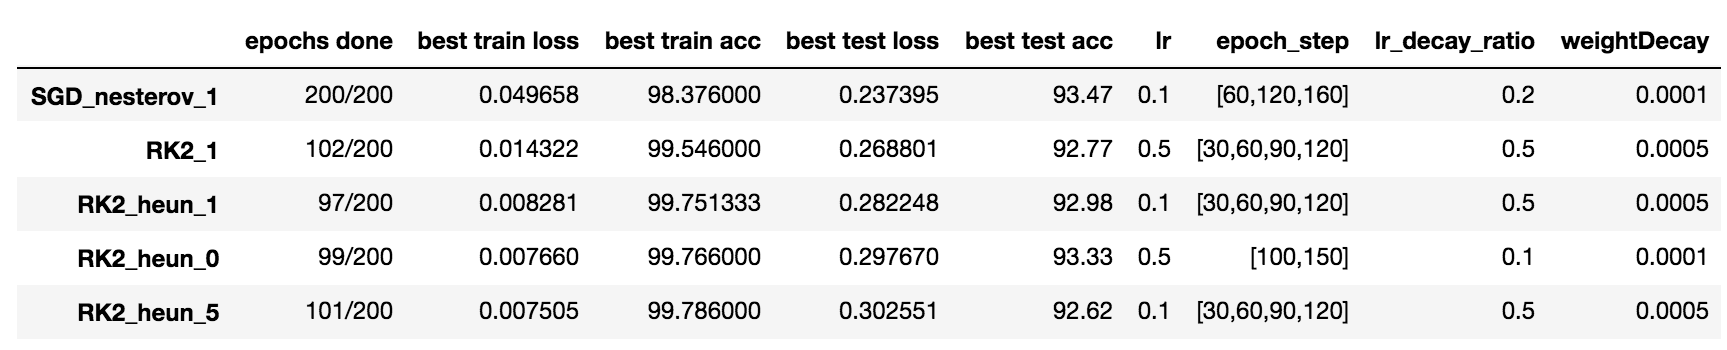
\includegraphics[scale=0.5]{wideresnet28_test_loss.png}
% \caption{WideResNet-28 CIFAR-10 Test loss}
% \end{figure}

% \begin{figure}[htb]
% 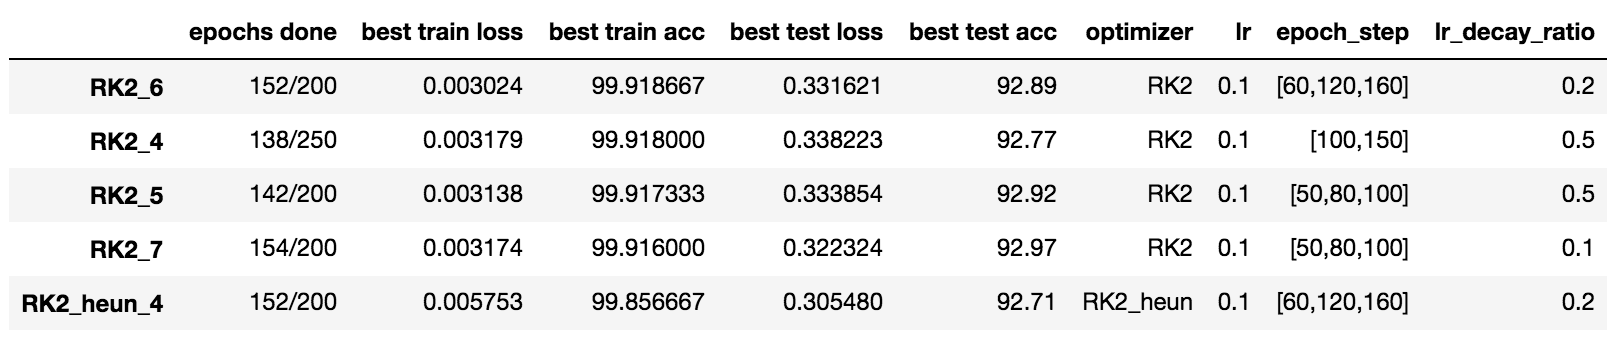
\includegraphics[scale=0.5]{wideresnet28_train_acc.png}
% \caption{WideResNet-28 CIFAR-10 Train Accuracy}
% \end{figure}

%%% Local Variables:
%%% mode: latex
%%% TeX-master: "main"
%%% End:
